\documentclass[a4paper, 12pt, oneside]{scrbook}
\usepackage[margin=2.5cm, bindingoffset=0.5cm]{geometry}

\usepackage[utf8]{inputenc}
\usepackage[hidelinks]{hyperref}
\usepackage{subcaption}
\usepackage{graphicx}
\graphicspath{{./images/}}
\usepackage{wrapfig}
\usepackage{float}
\usepackage{xcolor}
\usepackage[ngerman]{babel}
\usepackage{csquotes}
\usepackage[parfill]{parskip}
\usepackage[backend=bibtex, style=numeric, sorting=none]{biblatex}
\addbibresource{thesis.bib}
\usepackage{algorithm}
\usepackage{algpseudocode}
\renewcommand{\listalgorithmname}{Liste der Algorithmen}
\floatname{algorithm}{Algorithmus}
\captionsetup{format=plain, font=small}
\raggedright

\begin{document}

\definecolor{htwgreen}{RGB}{118,185,0}
\begin{titlepage}
\begin{center}

\includegraphics{logo.jpg}
\linebreak[4]
\linebreak[4]
\linebreak[4]
\linebreak[4]
\textbf{\Large\color{htwgreen}Erstellung eines interaktiven, 3D Höhenmodells des Mars auf Grundlage von MOLA Daten}
\linebreak[4]
\linebreak[4]
\linebreak[4]
Abschlussarbeit
\linebreak[4]
\linebreak[4]
zur Erlangung des akademischen Grades:
\linebreak[4]
\linebreak[4]
Bachelor of Science (B.Sc.)
\linebreak[4]
\linebreak[4]
an der
\linebreak[4]
\linebreak[4]
Hochschule für Technik und Wirtschaft (HTW) Berlin
\linebreak[4]
Fachbereich 4: Informatik, Kommunikation und Wirtschaft
\linebreak[4]
Studiengang Angewandte Informatik
\linebreak[4]
\linebreak[4]
\linebreak[4]
1. Gutachter: Prof. Dr.-Ing. Thomas Jung
\linebreak[4]
2. Gutachter: Michael Mario Droste, M.Sc.
\linebreak[4]
\linebreak[4]
\linebreak[4]
\linebreak[4]
\linebreak[4]
Eingereicht von Tim Oelkers
\vfill
\today
\end{center}
\end{titlepage}
\frontmatter
\chapter{Kurzbeschreibung}
\tableofcontents
\listoffigures
\let\defaultclearpage\clearpage
\let\clearpage\relax
\listofalgorithms
\let\clearpage\defaultclearpage
\mainmatter
\chapter{Einführung}

\section{Motivation}
Der Mars als unser Nachbarplanet ist, aufgrund seines Klimas und der Nähe, der am Besten für eine Besiedelung geeignetste, erdähnliche Planet in unserem Sonnensystem. Auch ist er das Ziel unzähliger Forschungen, insbesondere zu der Frage ob Leben außerhalb der Erde existieren kann. Aktuell findet ein kleiner Wettlauf zum Mars statt. Der \textit{Perseverance Rover} der NASA landete am 18.02.2021 und \textit{Tianwen-1} aus China am 14.05.2021. Des Weiteren ist derzeit die Raumsonde \textit{al-Amal} aus den Vereinigten Arabischen Emiraten in der Mars-Umlaufbahn, eine Landung ist allerdings nicht vorgesehen. Des Weiteren planen auch Japan und Indien eine Rover Mission in den nächsten Jahren. Allerdings sind Mars-Missionen kein einfaches Unterfangen, von den letzten 50 Mission schlugen 29 zumindest teilweise fehl\footnote{\url{https://de.wikipedia.org/wiki/Chronologie_der_Marsmissionen}}.Eine Visualisierung hat vor allem informative Gründe. Dieses Projekt versucht interessierten Menschen zum Beispiel die Probleme einer Mars-Besiedelung oder allein schon die Probleme einer Landung vor Augen zu führen. Vor allem, da zwar einige 2D Visualisierungen mit derselben Datengrundlage existieren, echte 3D Visualisierungen aber schwer zu finden sind.

\section{Zielstellung}
Im Zuge dieser Arbeit soll ein Prototyp geschaffen werden, welcher die Oberflächenstruktur des Mars in höchstem Detailgrad als 3D Modell darstellt. Der Nutzer soll möglichst ungehindert die Oberfläche aus verschiedenen Winkeln und Zoomstufen betrachten können. Ein kleines User Interface soll Informationen über den aktuellen Ort darstellen und den Nutzer bei der Navigation unterstützen.

Die Frage, die diese Arbeit mit dem Projekt zu beantworten versucht, ist, welche technischen Möglichkeiten existieren um mit dem Problem der Datenmenge (siehe Abschnitt \ref{datenmenge}) fertig zu werden und ob eine so detailgetreue Darstellung aus Nutzersicht überhaupt sinnvoll ist. Vor allem, da eine Verbesserung des Detailgrades natürlich immer mit einer Verschlechterung der Performance in Verbindung gesetzt werden muss. Hierbei sollen verschiedene Möglichkeiten, sowohl verlustfrei als auch verlustbehaftet, implementiert und durch quantitative als auch qualitative/empirische Methoden evaluiert werden.

\section{Aufbau der Arbeit}
% Link zum Prototyp und seinem Quellcode
% bechreibe, dass keine Garnatiee für die ständige Verfügbarkeit gegegen werden kann, Anleitung zum selbst kompilieren dazu packen (Link zum Download der Daten)
% Link zur virtuellen Version dieses Dokuments

\chapter{Grundlagen}

\section{Datenquellen}
Die Datengrundlage für dieses Projekt sind Daten des Mars Orbiter Laser Altimeter (MOLA), einem Höhenmessgerät an Bord des 
               

% Beschreibe die MOLA Mission und mit welchen Instrumenten sie erfasst wurden

% Beschreibe die Parameter (Auflösung, Datengröße, Genauigkeit (horizontal/vertikal))
% Beschreibe das Datenformat und Unterschiede / Vor- und Nachteile

%% https://pds-geosciences.wustl.edu/missions/mgs/megdr.html vs. https://astrogeology.usgs.gov/search/details/Mars/GlobalSurveyor/MOLA/Mars_MGS_MOLA_DEM_mosaic_global_463m
%% entscheide dich für die 2., auch wenn du das Format des 1. besser findest <-- da beim 1. Daten fehlen und das Mapping Auf Kugel dann schwierig wird
%% beschreibe, warum das Format nicht gut ist -> beschreibe Aufbau von TIFF Dateien (Container-Format, Daten an verschiedenen Stellen in der Datei) -> decoder benötigt

\section{OpenGL}
% Grundlagen: nur Interface, verschiedene Implementationen in Form von Driver
% existiert auch WebGL ← Unterschiede und Gemeinsamkeiten, z.B. 
% Erklärung Shader Pipeline
% Erklärung Kommunikation mit Shader (Attribut vs Uniform)
% Koodinaten Systeme -> wie verlaufen die Achsen (positive x-Achse nach rechts, positive y-Achse nach oben und positive z-Achse in den Bildschirm hinein)

\section{Datenreduzierung}

\subsection{Datenmenge}\label{datenmenge}

\subsection{Verlustfrei}

\subsection{Verlustbehaftet}
% Abschnitt, der erstmal die vollständige Datengröße beschreibt
% außerdem ist es ein Rasterformat, also feste Abstände zwischen einzelnen Datenpunkten

% verlustfrei: alles was nicht im Sichtbereich der Kamera liegt (Frustum Culling) und alles, was durch andere Dinge verdeckt wird (Occlusion Culling) -> andere Seite des Globus
% dazu Unterteilung der Welt in Abschnitte (chunks) und nur Anzeigen der Abschnitte, welche den Sichtbreich auch nur ansatzweise schneiden und nicht vollständig durch andere Abschnitte verdeckt sind
% verlustbehaftet: 
% hier ausnutzen, dass zum Beispiel bei geringen Zoomstufen Unterschiede in den Daten nicht mehr wahrgenommen werden können
% Außerdem: Entfernung von Redundanzen -> da Rasterformat , hier ist es abhängig von der Komplexität des Terrains,

% Redukttion der Datenmenge in festgelegten Schritten (stride), systemetaische Reduktion
% Reduktion der Datenmenge abhängig vom umliegenden Terrain -> ähnliche vertices müssen nicht wiederholt werden,
% gerade bei natürlichen Daten gibt es sehr ähnliche Pubkt

% eine Plane besteht zwar auf 4 Eckpunkten, allerdings muss sie in OpenGL Primitives zerlegt werden -> dies sind normalerweise Dreiecke, also 6 Eckpunkte, da ja jeder Eckpunk auch Teil des benachbartenn PLane ist, wird insgesamt ein Eckpunkt 6 mal wiederholt (siehe kleine Grafik) -> also wird bei der Erzeugung des Modell eine Indexierung vorgenommen, einfach eine Liste mit Indexen die eine die Liste mit den Vertex-Daten referenziert ->
% bei der systematischen Reduktion ist das kein Problem, die Indixierung des Raster Modells bleibt erhalten, nur die Abstände zwischen den Vertices erhöhen sich

% erwähne die Formel um aus einem 1D Array ein 2D Array zu erstellen

% bei der asymetrischen Reduktion kann nicht mehr aus dem 1D Vertex-Format auf eine Indexierung geschlossen werden, also muss hier ein 2D Format gesendet werden was die entfernen
% Vertex-Daten kennzeichnet
\chapter{Anforderungsanalyse}\label{chapter3}

\section{Zielgruppe}
Die Zielgruppe dieses Projekts lässt sich relativ schwer eingrenzen. Es betrifft vor allem Personen mit Interesse in Raumfahrt oder dem Weltraum allgemein. Wichtig ist, das diese Personen keinen Bezug zur Informatik aufweisen müssen und zum Beispiel die Bedienung des User Interface daher kein Spezialwissen erfordern darf. Auch die Visualisierung der Oberfläche muss ohne Vorkenntnisse verständlich sein und dabei trotzdem noch die eigentliche Oberfläche korrekt und realitätsnah repräsentieren. Eine weitere mögliche Zielgruppe sind Schüler und Studenten, welche die Visualisierung unter anderem für Forschungszwecke nutzen können. Das Jet Propulsion Laboratory (JPL), einem Institut der NASA, welches sich auf die Entwicklung von Raumsonden und Satelliten spezialisiert, nutzt intern eine Visualisierung namens Mars Trek (siehe Abschnitt \ref{marsTrek}) bereits um Landeziele für Marsmissionen zu finden und plant dies auch für die Auswahl zukünftiger bemannter Erkundungsmissionen zu nutzen\cite{marsTrek}. Des Weiteren könnte eine Visualisierung in den Forschungsbereichen Astronomie und insbesondere Geologie nützlich sein.

\section{Ist-Zustand}\label{istZustand}
Bevor Anforderungen definiert werden können, müssen alternative Visualisierungen in Betracht gezogen werden. Dieses Projekt soll sich dabei an gängigen Visualisierungen orientieren und versuchen deren Schwächen zu vermindern. Zu beachten ist, dass eine Limitierung auf kostenlose Anwendung vorgenommen, um einen besseren Vergleich für dieses Projekt zu erhalten. Eine bekannte Visualisierung des JPL nennt sich Mars Trek\footnote{https://trek.nasa.gov/mars/index.html} und wurde im Jahr 2015 veröffentlicht. Es ist ein web-basiertes Tool um verschiedene Daten, gesammelt aus unterschiedlichen NASA Missionen, in einer interaktiven 3D Visualisierung zu visualisieren. Eine weitere Visualisierung versteckt sich in der Desktop Version von Google Earth\footnote{https://www.google.com/earth/versions/\#earth-pro}. Google Earth ist wohl einer der populärsten Visualisierungen von Geodaten, insbesondere für die Erde. Und auch wenn es der Name nicht vermuten lässt, befindet sich in der Download-Version seit dem Jahr 2009 auch eine Visualisierung des Mars. Im folgenden werden die Alternativen beschrieben und deren Stärken und Schwächen hervorgehoben.

\subsection{Mars Trek}\label{marsTrek}
Das erste, was bei der Anwendung negativ auffällt, sind die langen Ladezeiten, die noch vor der eigentlichen Visualisierung zu sehen sind. Diese liegen beim ersten Laden der Seite im zweistelligen Sekundenbereich bis zur Sichtbarkeit der Visualisierung und ungefähr doppelt so lang bis zum vollständigen Laden der Seite (siehe Abbildung \ref{marsTrekLoading} für ein durchschnittliches Laden). Nachfolgende Ladezyklen sind dann dank Cachings deutlich schneller, die Ladezeiten sind aber für ein anfangs sehr gering aufgelöstes 2D Bild trotzdem sehr hoch. Zwar sind dadurch anfangs keine visuellen Artefakte zu sehen, diese werden dann beim Bewegen der Kamera jedoch sichtbar, sodass die Nützlichkeit in Frage gestellt werden kann.

\begin{figure}[H]
  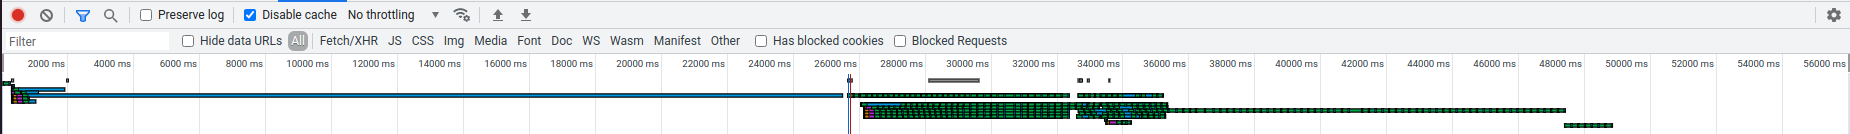
\includegraphics[width=\textwidth,keepaspectratio]{marsTrekLoading.png}
  \caption{Ladezeiten der Mars Trek Anwendung bei 100 Mbit/s auf Mittelklasse-PC}
  \label{marsTrekLoading}
\end{figure}

Initial wird man von der Anwendung mit einer 2D Ansicht des Mars mit Daten der Viking Missionen begrüßt (siehe Abbildung \ref{marsTrekStart}). Zusätzlich wird dem Nutzer ein Tutorial angeboten, was auf eine relativ komplexe Anwendung schließen lässt. Die Anwendung sieht auf den ersten Blick allerdings sehr übersichtlich aus und die einzelnen Menüs lenken nicht von der eigentlichen Visualisierung ab.

\begin{figure}[H]
  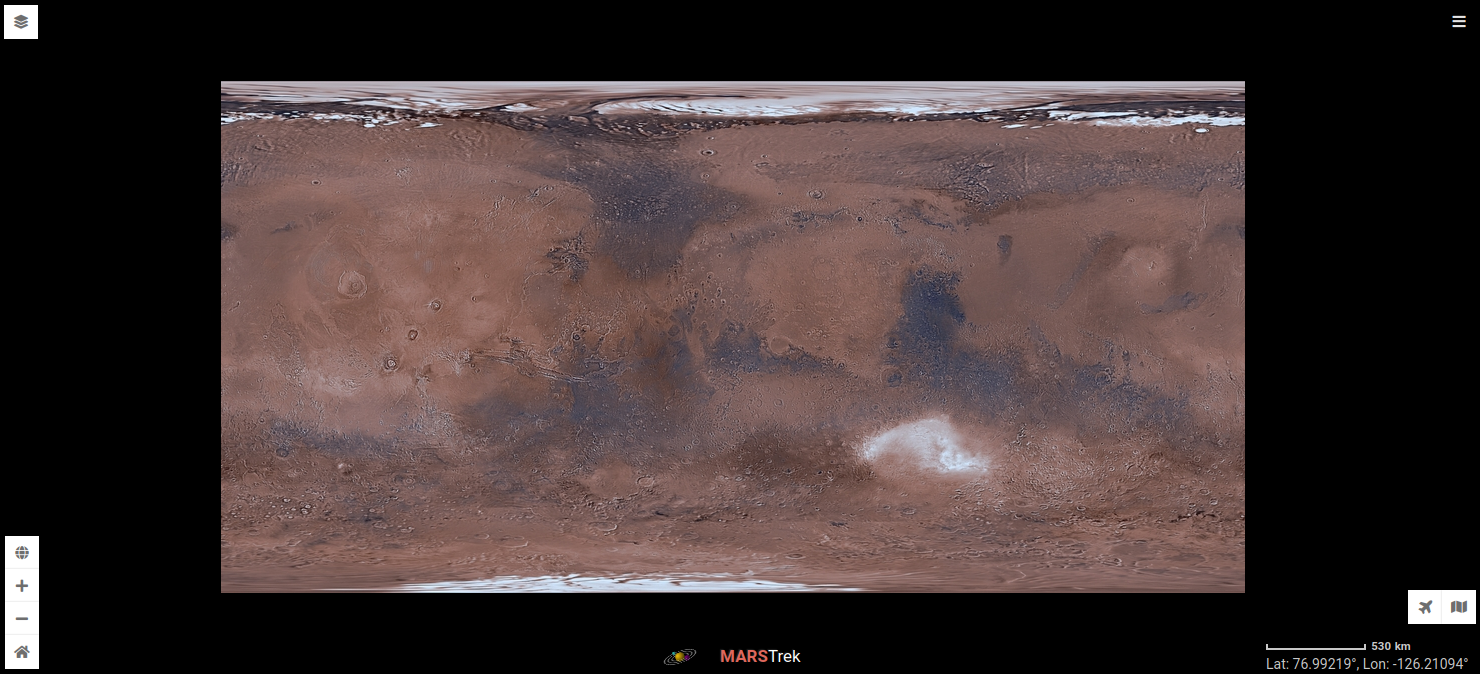
\includegraphics[width=\textwidth,keepaspectratio]{marsTrekStart.png}
  \caption{Initiale Ansicht der Mars Trek Anwendung}
  \label{marsTrekStart}
\end{figure}

Dabei befindet sich in der oberen linken Ecke ein Menü, mit dem man die verwendeten Daten auswählen kann. Unter anderem können auch MOLA Daten gewählt werden, bei denen die Höhenwerte als Farbwerte kodiert sind, ein Punkt, der auch mit diesem Projekt genutzt werden soll. Negativ fällt hier auf, dass die UI hier sehr überladen ist. Es stehen über 2000 verschiedene Datensätze zur Auswahl und die Filter nach Mission, Messinstrument, Koordinaten oder nach verschiedenen (Sub-)Kategorien ist für den Laien schwer verständlich. Auch sind nicht alle Daten für alle Flächen verfügbar, sodass teilweise nicht das gewünschte Resultat zustande kommt und sich verschiedene Ebenen nicht vollständig überlappen. Hier ist zwar ein Zeichentool vorhanden, mit dem man Ausschnitte auf der Karte definieren kann, die als weiterer Filter genutzt werden können, dies ist aber auch nicht intuitiv verständlich. 

In der unteren linken Ecke befindet sich ein Menü, mit dem man unter anderem die Projektion wechseln kann. Hier stehen eine Projektion der beiden Pole, eine globale 2D Ansicht und eine Projektion als Kugel zur Auswahl. Hier könnte das Wechseln noch intuitiver gemacht werden, da die Ansicht als 3D Modell das Highlight der Anwendung sein sollte und die derzeitige Lösung sehr versteckt ist. Des Weiteren lässt sich in dem Menü der Zoom in kleinen Schritten vergrößern und verkleinern, was durch ein Scrollen des Mausrads deutlich leichter fällt. Auch existiert dort ein Button, um die Visualisierung wieder auf den Startzustand zurückzusetzen. Wenn die 3D Ansicht ausgewählt wurde, ist zusätzlich ein Button eingeblendet, mit dem man zwischen einer statischen Kameraansicht und einer frei bewegbaren Kamera wählen kann. Die statische Kamera kann genutzt werden, um in einem festen Abstand um den Planeten zu rotieren und die dynamische Kamera bewegt sich entlang der Blickrichtung und lässt sich durch die bekannten Steuerungstasten WASD oder Pfeiltasten steuern. Dadurch lassen sich bestimmte Orte viel genauer ansteuern, was ein deutlicher Pluspunkt ist.

In der oberen rechten Ecke befindet sich ein allgemeines Menü, in dem verschiedene nützliche Tools vorhanden sind, unter anderem um Distanzen und Höhenprofile zu messen, eine 3D Datei zu erstellen oder die Winkel zur Sonne über die Zeit zu berechnen. Auch diese Tools sind für den durchschnittlichen Nutzer sicherlich nicht besonders nützlich. Auch sind diese Tools nicht in der 3D Ansicht vorhanden, was aus der reinen Machbarkeit keinen Sinn ergibt. Des Weiteren sind hier allgemeine Informationen über die Anwendung, die Entwickler, Release Notes oder Systemanforderungen zu finden. Letzte belegen, dass die Anwendung mit WebGL programmiert wurde und dass die 3D Ansicht einen relativ neuen Browser benötigt.

In der unteren rechten Ecke existiert zum einen eine Möglichkeit, zu bestimmten Koordinaten zu springen. Zum anderen befindet sich dort eine Übersicht, welche den Datensatz auf den einzelnen Ebenen anzeigt. Auch kann hier die Sichtbarkeit einzelner Ebenen angepasst werden, falls diese sich überlappen sollen. Abschließend befindet sich dort eine Skala, die die Längen in Kilometern einer Länge auf dem Bildschirm zuordnet und die Koordinaten des Punktes unter dem Mauszeiger. Hier wird allerdings die Angabe der Höhe vermisst, welche sich wunderbar in das Menü integrieren würde. Generell scheint es keine Möglichkeit zu geben, sich mehr Informationen zu einem bestimmten Punkt anzeigen zu lassen, was für bestimmte geografische Features durchaus sinnvoll sein könnte.

Alles in allem ist die Anwendung ein sehr gutes Beispiel und das generelle Design und viele Features können übernommen werden. Allerdings soll gerade im Hinblick auf eine breitere Zielgruppe die Komplexität verringert werden, indem einige Features bewusst nicht übernommen werden. Auch sollte die User Experience (UX) in einigen Menüs überdacht werden. Idealerweise sollte auch auf die langen Ladezeiten verzichtet werden.

\subsection{Google Earth}
Ein Negativpunkt bei dieser Anwendung ist die Tatsache, dass die Web-Version eine Visualisierung des Mars nicht unterstützt. Ein Download ist immer ein weiterer Schritt, den viele Nutzer, welche schnell eine Visualisierung betrachten möchten, nicht unbedingt gehen möchten. Auch hier sollte das Web die technischen Möglichkeiten geben, alle existierenden Features umzusetzen. Und auch bei dieser Anwendung wird man als erstes mit einem sehr textlastigem Tutorial und anschließend von einer sehr umfangreichen Anwendung, mit Blick auf die Erde, begrüßt (siehe Abbilding \ref{googleEarthStart}).

\begin{figure}[H]
  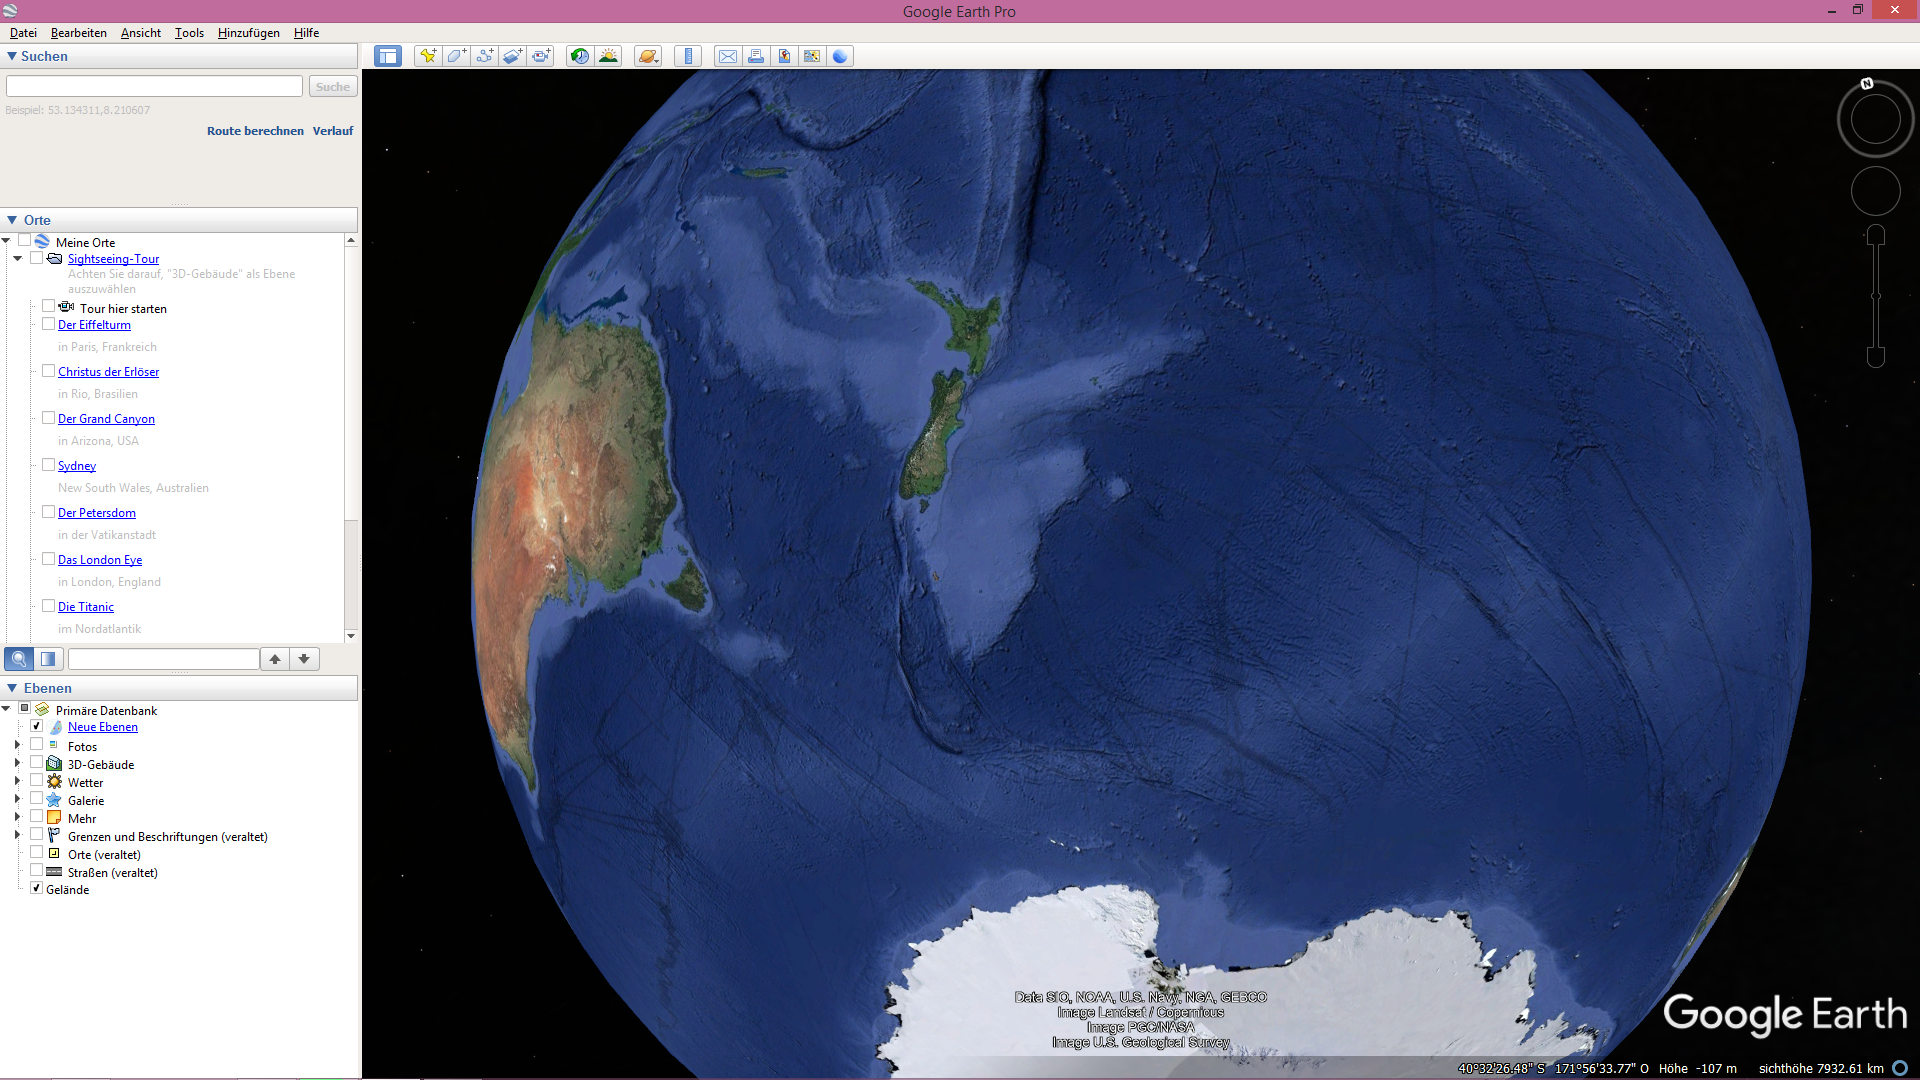
\includegraphics[width=\textwidth,keepaspectratio]{googleEarthStart.png}
  \caption{Initiale Ansicht der Google Earth Anwendung}
  \label{googleEarthStart}
\end{figure}

Hier ist nicht auf Anhieb ersichtlich, wie man die Visualisierung auf den Mars umstellen kann. Es befindet sich die Standard-Windows Menüleiste in der oberen linken Ecke, doch dort sind die Optionen sehr begrenzt. Zusätzlich befindet sich darunter eine weitere Menüleiste, die einige Funktionen aus der eigentlichen Menüleiste besonders dupliziert und so besonders hervorhebt. In den Menüs befinden sich unter anderem verschiedene Tools wie Entfernungsmesser, GPS oder auch ein Flugsimulator, mit dem man die Oberfläche in sehr kreativer Weise erkunden kann. Dies ist ein großer Pluspunkt, allerdings können die wenigsten ein Flugzeug intuitiv steuern und natürlich überschreitet dies den geplanten Projektrahmen bei weitem. Des Weiterem können verschiedene Elemente in der Visualisierung an- und ausgeschaltet werden, unter anderem ein realistische Beleuchtung per Sonne zu verschiedenen Tageszeiten. Auch eine realistische Wasseroberfläche und Atmosphäre, zusammen mit dem realgetreuen Sternenhimmel im Hintergrund, verstärken den Realitätsgrad in sehr großer Weise. Des Weiteren sind Ansichten wie ein Gitternetz mit Breiten- und Längenangaben und eine Minimap in der Ecke sehr hilfreich bei der Navigation. Weitere Menüpunkte dienen zum Wechseln zwischen Google Maps oder der Web-Version. Ein Wechsel von einer Download-Version zum Browser ist hierbei fragwürdig, vor allem da alle Funktionen der Web-Version auch in dieser Version vorhanden sind. Ein etwas kurioses Problem verbirgt sich hinter dem Menüpunkt ''Regionating durchführen''. Zum einen ist nicht verständlich, was man mit dem sich öffnenden Fenster verwirklichen kann, zum anderen lässt sich dieses Fenster einfach nicht mehr schließen, da die entsprechenden Buttons deaktiviert wurden. Warum so ein Usability-Problem bei einer so bekannten Anwendung einer so bekannten Firma beim Testen nicht entdeckt wurde ist nicht verständlich.

Schlussendlich findet man den Button zum Wechseln des Planeten unter den Menüpunkten ''Ansicht'' und dann ''Erkunden'', eine Wahl, die auf den ersten Blick nicht verständlich erscheint. Sobald man es geschafft hat, die Anwendung auf die Mars Visualisierung umzuschalten, fällt auf, dass gar keine 3D Höhendaten angezeigt werden, sondern Kamerabilder verschiedenster Marsmissionen als Textur auf eine Kugel projiziert wurden. Hierbei fällt auf, dass nicht immer die gleichen Daten für alle Flächen vorhanden sind und so ein Mix aus verschiedenen Datenquellen genutzt wird. Dies führt zu einem etwas schlechterem visuellen Eindruck (siehe Abbildung \ref{googleEarthMars}).

\begin{figure}[H]
  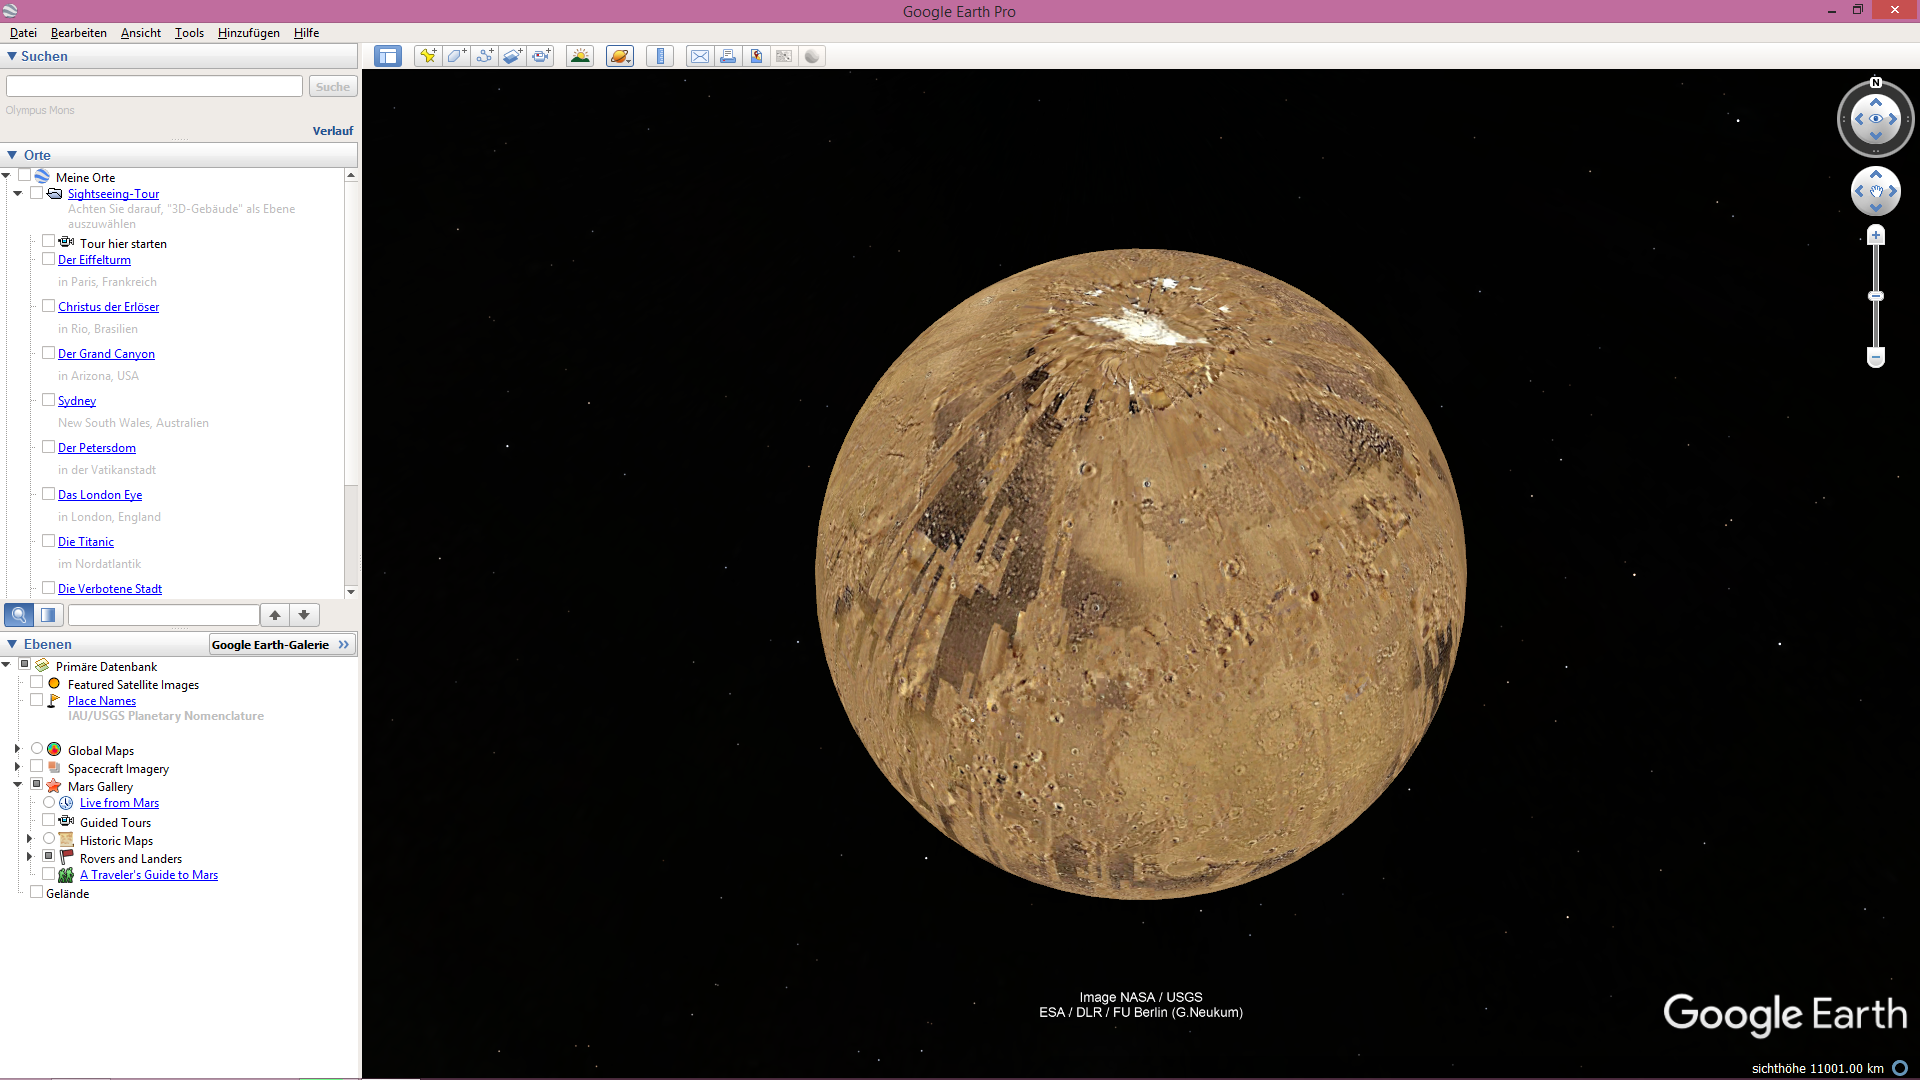
\includegraphics[width=\textwidth,keepaspectratio]{googleEarthMars.png}
  \caption{Initiale Mars Visualisierung der Google Earth Anwendung}
  \label{googleEarthMars}
\end{figure}

Auch diese Anwendung nutzt das Konzept von Ebenen um verschiedene Daten auf dem Globus gleichzeitig anzuzeigen. Hier wird der Fokus aber mehr auf verschiedene Dinge gelegt, welche sich in vollständig in die Visualisierung integrieren (z.B. Ortsnamen, Mars Rover oder Fotos bestimmter Marsmissionen). Hier findet man dann auch die Checkbox ''Gelände'', welche eine echte 3D Höhendarstellung ermöglicht. Der wahrscheinlichste Grund, warum dies standardmäßig deaktiviert ist, ist, dass weiterhin Satellietenbilder auf dem Globus angezeigt werden und diese durch eine 3D Darstellung verzerrt werden. Dies verschlechtert die Kantenbildung zwischen benachbarten Satelietenbildern noch weiter. Eine Möglichkeit die Bodendarstellung auf eine weniger realistische Darstellung zu wechseln ist nicht vorhanden. Ein weiteres Problem ist das Panel ''Orte'' auf der linken Seite. Es ist definitiv für die Erde ausgelegt und erlaubt es dem Benutzer zu verschiedenen Sehenswürdigkeiten wie dem Eifelturm oder dem Petersdom zu springen, ein Feature, was auf dem Mars völlig fehl am Platz ist. Immerhin ist die Suchleiste in der oberen linken Ecke funktional und man kann zu bestimmten geographischen Featuren wie dem Olympus Mons springen.

Auf der anderen Seite befindet sich verschiedene Möglichkeiten die Kamera zu bewegen. Zum einen ermöglichen sie die Rotation um den stationären Mars in x- und y-Richtung. Dies ist ebenfalls mit den Pfeiltasten und WASD und durch Ziehen der Maus in eine bestimmte Richtung möglich, was eine deutlich intuitive Steuerung darstellt. Zum anderen ermöglicht es die Rotation des Globus um die z-Achse (Rolling), was nachfolgende Interaktionen sehr verwirrend macht. Eine feste Positionierung des Nordpols nach oben ist eine allgemein bekannte Darstellung (auch bei physischen Globen) und ein Ändern dieser Darstellung sollte den wenigsten Nutzern von Vorteil sein. Des Weiteren ist auch hier eine Möglichkeit gegeben, den Zoom per Mausklick anzupassen. Da dies per Mausrad jedoch deutlich einfacher ist, ist auch hier der Nutzen in Frage gestellt. Eine frei im Raum bewegliche Kamera ist nicht vorhanden (mit Ausnahme des Flugsimulators), sodass bestimmte Orte teilweise recht umständlich erreicht werden können. In der unteren rechten Ecke befinden sich noch die Koordinaten der Position des Mauszeiger auf dem Planeten und eine Angabe, in welcher Höhe sich die Kamera über dem Erdboden befindet. Dies ist eine sehr nützliche Information um Abstände einordnen zu können. Allerdings wird auch hier die Höhenangabe des Punktes auf dem Planeten nicht angezeigt. Auch das übergroßes Logo (15\% der Gesamtbreite) in der Ecke ist etwas ablenkend und hat keinen funktionalen Nutzen.

Alles in allem ist auch diese Anwendung sehr komplex und für Laien nicht als Visualisierung des Mars erkenntlich. Es kommt auch das Gefühl auf, als ob diese Anwendung ursprünglich nicht für die Visualisierung weiterer Planeten gedacht ist, ein Punkt, der wegen des Namens sehr wahrscheinlich scheint. Die Benutzerführung sollte verbessert werden und doppelte Wege ein bestimmtes Ziel aus Nutzersicht zu erreichen vermieden werden. Ein großer Pluspunkt dieser Anwendung ist der unglaublich hohe Realitätsgrad mit hochaufgelösten Bildern bei hohen Zoomfaktoren und den verschiedenen Möglichkeiten Wetter, Sonne, Wasser und ähnliche Dinge physikalisch korrekt in die Visualisierung einfließen zu lassen. Dieser Realitätsgrad wird jedoch durch den Mix aus verschiedenen Satellietenbildern stark gestört.

\section{Anforderungen}
Auf Grund des Prototypen-Charakters dieses Projekts besteht eine geringere Priorisierung bei den funktionalen und nicht-funktionalen Anforderungen. Es sollen möglichst viele verschiedenen Möglichkeiten zur Datenreduzierung (siehe Abschnitt \ref{datenreduzierung} implementiert und evaluiert werden. Die Anwendung soll dennoch einen Nutzen erfüllen um die Evaluation so realistisch wie möglich zu gestalten. Auch hilft dies dabei, die Korrektheit der Implementierungen zu verifizieren, wenn eine vollständige Visualisierung mit verschiedenen Features vorhanden ist. Um die konkreten Anforderungen zu ermitteln, wurden diverse Personen aus der Zielgruppe nach ihren Wünschen befragt. Aus diesen Wünschen wurden die Features priorisiert, die von den meisten Personen gewünscht wurden. Des Weiteren wurden die Stärken der bisher analysierten Visualisierungen in Betracht gezogen und in die Anforderungen integriert. Bestimmte Features, welcher im gegebenem Projektzeitraum nicht umsetzbar waren, wurden dabei im voraus verworfen.

\subsection{Funktional}
Die wichtigste funktionale Anforderung ist eine realistische Darstellung des Mars mit den beschriebenen MOLA Daten. Dabei soll eine reine 3D Darstellung gewählt werden, bei der die Höhenwerte realistisch den Globus verformen, das Anzeigen einer Textur der Oberfläche auf einer 3D Kugel soll nicht genutzt werden. Der Hauptgrund dafür ist die realistischere Darstellung, besonders bei hohen Zoomstufen. Des Weiteren hilft es dabei, die Datenreduzierung besser zu evaluieren, da das Generieren einer Textur aus den Daten eine einmalige Tätigkeit darstellt und auch keinem Zwang der Datenreduzierung unterliegt. Es kann unabhängig von der Laufzeit beliebig lange dauern und die Größe von einzelnen Texturen ist zwar durch die OpenGL Implementation limitiert, sie kann aber leicht in einzelne kleinere Texturen aufgeteilt werden. Die Gesamtdatenmenge ist dabei nicht vergleichbar mit der Datenmenge von Modellen mit individuellen Höhenwerten. Ein nicht repräsentativer Test auf eigener Hardware zeigte, dass ein Aufteilen der Textur in 4 Abschnitte bereits ausreichen würde um sie in höchster Auflösung anzeigen zu können. Und Techniken wie das frustum- oder occlusion-culling, die zur Laufzeit die Datenmenge reduzieren, sind dabei nicht notwendig. Neben der Projektion der Daten in eine Kugelform soll auch die flache Darstellung ermöglicht werden, bei der allerdings dennoch 3D Koordinaten genutzt werden. Dies soll, anders als bei der MarsTrek Anwendung, allerdings nicht der Standard sein und vom Benutzer bewusst ausgewählt werden müssen. Ein möglicher Nutzen von einer flachen Darstellung ist die bessere Einschätzung von Entfernungen und geraden Linien, was auf einer Kugel oft nicht intuitiv ist.

Für die Darstellung der Oberfläche soll eine schematische Darstellung genutzt werden, bei der keine weiteren Datenquellen notwendig sind. Die Wahl fiel dabei auf eine topographische Darstellung, bekannt aus Atlanten, bei der der Farbwert abhängig vom Höhenwert ist. Der Farbwert wird dabei aus einem vordefiniertem Farbbereich linear interpoliert. Der Hauptgrund für diese Wahl ist vor allem der begrenzte Projektzeitraum. Ein Einbinden von weiteren Quellen zur Bestimmung der Oberflächenbeschaffenheit (z.B. Gesteinsart oder Eis) hätte die Komplexität noch weiter erhöht und wurde in diesem Projekt als nicht durchführbar eingestuft. Die verwendete Farbskala muss dem Benutzer auch mitgeteilt werden, eine entsprechende Übersicht welche Farbe zu welchem Höhenwert gehört, muss also angezeigt werden. Dabei sollen die Ränder der Skala vom Benutzer konfigurierbar sein. Der Nutzer soll also effektiv bestimmen können, welcher minimale und maximale Höhenwert für die lineare Interpolation genutzt wird. Welche Farben genutzt werden, muss noch evaluiert werden, der Nutzer soll diese aber nicht ändern können, da dafür kein Use-Case gefunden wurde und es die Komplexität unnötig erhöht. Standardmäßig soll ein minimaler und maximaler Wert gefunden werden, der eine möglichst gleichmäßige Farbverteilung ermöglicht. Besondere Extreme, wie zum Beispiel der Olympus Mons, sollten dabei außen vor gelassen werden, da es die Skala sonst stark in eine Richtung verzerrt und die Farbverteilung so stark verringert.

Für die Interaktion mit dem Mars sollen verschiedene Möglichkeiten genutzt werden, die möglichst intuitiv sind und keiner textuellen Erklärung benötigen. Zum einen betrifft das die Steuerung der Kamera. Dies ist ein wichtiger Aspekt im Design des Prototypen und es muss darauf geachtet werden, dass die Bewegung sowohl aus der Ferne flüssig ist, also auch bei hoher Zoomstufe noch präzise bestimmte Orte betrachtet werden können. Zum einen soll hier eine stationäre Kamera implementiert werden, die in einem festen Abstand um den Globus rotiert. Die Rotation soll dabei mit der Maus erfolgen und auch das Ändern des Abstands, höchstwahrscheinlich mit dem Mausrad, ermöglichen. Zum anderen soll eine frei bewegliche Kamera implementiert werden, die mit der Tastatur frei in alle 6 Richtungen gesteuert werden kann. In dieser Konfiguration soll man sich mit der Maus umschauen können und sich dann entsprechend der Blickrichtung bewegen können. Diese Kamera muss in der flachen Projektion auch erzwungen werden, da hier natürlich eine Rotation um den Globus nicht möglich ist. Eine weitere wichtige Interaktion soll das Erhalten von Informationen zu bestimmten Orten darstellen. Dabei soll der Benutzer auf einen Punkt auf dem Mars klicken können und dann zumindest die Koordinaten und den exakten Höhenwert angezeigt bekommen. Hier sollte idealerweise der Höhenwert in verschiedenen, vom Benutzer konfigurierbaren Einheiten angezeigt werden um die Zielgruppe noch weiter zu erhöhen. Standardmäßig sollen Meter oder Kilometer als Einheit genutzt werden.

Das Anzeigen von weiteren Informationen ist fakultativ, hier könnte man zum Beispiel auf benannte geologischen Features zurückgreifen, welche von der \textit{Working Group for Planetary System Nomenclature} bereitgestellt werden. Diese werden in einer Datenbank bereitgestellt, welche unter anderem deren Position und Durchmesser beinhaltet, sodass eine Integration machbar wäre\footnote{https://planetarynames.wr.usgs.gov/AdvancedSearch}. Weitere fakultative Anforderungen sind Features aus den analysierten Alternativen, die als hilfreich bei der Navigation eingestuft wurden. Hierzu zählt zum Beispiel das Gitternetz mit Längen- und Breitenangaben, sowie die Möglichkeit zu bestimmten Koordinaten zu springen. Auch wenn bei Darstellung der Oberfläche dieser Anwendung nicht realitätsnah werden soll, könnte man den Realitätsgrad dennoch deutlich erhöhen. Besonders die Google Earth Anwendung hat dies in sehr guter Weise gezeigt und Features wie eine korrekte Simulation der Sonne mit Licht- und Schatteneffekten zu bestimmten Tageszeiten oder einen realistischen Sternenhimmel im Hintergrund verstärkten die Immersion stark. Eine weitere fakultative Anforderung ist die Integration weiter Datenquellen. Diese Anwendung soll, wenn möglich, möglichst unabhängig von der Datenquelle sein und eine Integration weiterer Datenquellen, inklusive Auswahl durch den Benutzer, ermöglichen. Gute Alternativen sind hier unter anderem Höhendaten des Mondes (z.B. LOLA mit 8GB Rohdaten) oder der Erde (z.B. SRTM mit über 100Gb Rohdaten). Das Konzept von Ebenen, was in den analysierten Alternativen zum Einsatz kam, soll hier explizit nicht verwendet werden, da es in allen Fällen als zu kompliziert und wenig vorteilhaft eingestuft wurde. Der Nutzer soll immer nur Daten eines einzigen Datensatzes angezeigt bekommen.

\subsection{Nicht-Funktional}\label{nichtFunktional}
Die nicht-funktionalen Anforderungen richten sich hauptsächlich an die Qualität der Visualisierung und die Performance. Hier ist es schwer, die formulierten Wünsche in konkrete Anforderungen umzuwandeln, da hier oft subjektive Dinge eine Rolle spielen. Auch lassen sich bestimmte Dinge wie die Performance einfach nicht in der gewünschten Qualität (z.B. in der Form x Frames Per Second (FPS) auf Hardware y) definieren. Insbesondere die Hardwareanforderungen können dabei auf Grund der Hardwarevielfalt nicht genau definiert werden. Eine Kernaussage ist, dass die Anwendung möglichst immer die höchste Datenauflösung anzeigt, die möglich ist. Wie bereits beschrieben (siehe Abschnitt \ref{datenmenge}) ist ein dauerhaftes Anzeigen der höchstmöglichen Datenauflösung auf normaler Hardware einfach nicht umsetzbar. Daher soll die Auflösung immer genau so hoch gewählt werden, dass eine dauerhafte Framerate von ungefähr 30 FPS erreicht wird. Die Framerate sollte möglichst genau getroffen werden, eine Abweichung darunter schadet der User Experience (UX), eine Abweichung darüber erlaubt eine Verbesserung der Datenauflösung. Hier ist also ein sehr starkes Ringen zwischen Performance und Qualität vorhanden. Der Wert wurde, anstatt der üblichen 60 FPS, nur auf ungefähr 30 FPS festgelegt, da die Visualisierung keine starken Bewegungen und somit keine flüssigen Übergange benötigt. Der Nutzer soll zwar die Kamera bewegen können, allerdings liegt der Fokus dabei immer noch auf der Visualisierung an sich.

Ein weiterer Aspekt ist, dass keine dedizierten Ladezeiten vorhanden sein sollen, in denen die Visualisierung nicht zu sehen ist. Dies wird häufig genutzt, um visuelle Ladeartefakte zu verstecken. Diese können zum Beispiel auftreten, wenn neue Abschnitte geladen werden müssen, nachdem der Benutzer die Kamerasicht verändert hat. Idealerweise soll auch auch ohne Ladezeiten der Nutzer nichts von der Trennung in Abschnitte mitbekommen und immer den Mars als Ganzes sehen. Dies kann zum Beispiel erreicht werden, in dem die Bewegung der Kamera antizipiert wird und Abschnitte, welche als nächstes geladen werden müssten, bereits vorgeladen werden.

Wichtig ist, dass die bisherigen nicht-funktionalen Anforderungen immer abhängig von der Hardware des Nutzer sind, da die Visualisierung auf Client-Seite durchgeführt wird. Es kann also kein einheitliches Performance-Konzept geben, welches für alle Nutzer geeignet ist. Zum einen können natürlich einzelne Parameter im voraus für verschiedene Performance-Klassen per Hand definiert werden. Da dafür allerdings eine umfassende Evaluation auf unterschiedlicher Hardware notwendig ist, ist der Zeitaufwand sehr groß. Eine Alternative ist es, zur Laufzeit bestimmte Parameter an die aktuellen Hardware anzupassen. Ein Problem bei beiden Ansätzen ist auch das Erfassen der aktuellen Hardware an sich. Auch ohne sich bereits auf eine Sprache oder Plattform festgelegt zu haben, gibt es meist keinen einheitlichen Weg diese zur Laufzeit zu erfassen. Natürlich könnte man den Nutzer nach der gewünschten Qualität fragen. Dieser Ansatz wird in der Realität sehr oft durchgeführt, allerdings soll die Zielgruppe kein Spezialwissen benötigen und Kenntnisse über die aktuelle Hardware sind nicht überall vorhanden. Ein Ansatz wäre es sich nicht auf die Hardware an sich zu konzentrieren, sondern zur Laufzeit die Auswirkungen zu messen und sich dementsprechend anzupassen. Man könnte zum Beispiel Parameter wie die Framerate als Indikator nutzen und dann zur Laufzeit auf Schwankungen reagieren. Alles in allem soll dieses Projekt als Prototyp dienen und ein Finetuning aller Parameter würde den Projektrahmen sprengen. Daher sind die bisher beschriebenen Anforderungen fakultativ und eher als ungefähre Richtwerte zu verstehen.

Eine Anforderung, auf die großen Wert gelegt werden soll, ist die Skalierbarkeit der Anwendung. Das Ziel dieses Projekts ist die Evaluation von verschiedenen Methoden zur Datenreduzierung. Dies soll idealerweise nicht von den verwendeten Daten abhängen und muss universell funktionieren. Die gesamte Anwendung, mit Ausnahme von Modulen die spezifische Datenformate interpretieren, muss also mit dieser Anforderung gestaltet werden. Ein Kernaspekt dieser Anforderung ist eine strikte Begrenzung von Arbeitsspeicher (RAM) und Grafikkartenspeicher (VRAM). Diese beiden Performancekriterien sind gut geeignet, die Qualität der Datenreduzierung zu beurteilen. Wichtig ist auch hier, dass der verwendete Datensatz keinen Einfluss auf die Anforderung hat, die gleichen Anforderungen müssen auch für einen Datensatz gelten, der mehrere hunderte Male größer ist. Als konkrete obere Grenze wurde Richtwerte an Mittelklasse Computer verwendet und bestehen aus 8 GB für den RAM und 4 GB für den VRAM. Eine Konsequenz, die sich aus diesen Anforderung ergibt ist, dass die Quelldaten niemals vollständig in den Arbeitsspeicher geladen werden dürfen (auch wenn es für MOLA Daten mit 2 GB ausreichen würde).

\chapter{Konzeption}

\section{Vorgehensmodell}
% Seite namens genmymodel für die Erstellung von UML Diagrammen
% diagrams.net für die Erstellung von Mock-Ups
% alleinige Durchführung des Projekts, inklusive Auftraggeber und Projektdurchführung die selbe Person, deshlab sollte einem formellen Vorgehen eine geringere Bedeutung zugedacht werden
% insbesondere agile Vorgehensmodelle machen wenig Sinn, da deren Vorteile, z.B. die Reaktion auf wechselnde Anforderungen oder die Auslieferung von Teilartefakten hier nicht notwendig sind
% strikte Einhaltung von inkrementellem Waserfallmodell, immer erst Planung, dann Entwicklung, dann Evaluation 
% da bei diesem Projekt einige Unsicherheiten im Zusammenhang mit der Datenmenge eistieren, ist ein inkrementelles Vorgehen sehr wichtig
% oft sollen bestimmte Prototypen angelegt werden und evaluiert werden, bevor weitere Funktionalitäten implementiert werden

\section{Programmiersprache}
Die Wahl der richtigen Programmiersprache ist mehr als nur reine Präferenz, da jede Sprache projektrelevante Eigenheiten hat. Im folgenden werden daher drei Programmiersprachen auf ihre Projekttauglichkeit evaluiert. Für dieses Projekt irrelevante Aspekte wie zum Beispiel Sprachfeatures oder Paradigmen fließen in die Bewertung nicht mit ein.

Der wichtigste Faktor aus Projektsicht ist das Zielsystem, auf die Software schlussendlich laufen wird. Sie bestimmt schlussendlich über die Zielgruppe und hat einen entscheidenden Einfluss auf die Reichweite des Projekts. Idealerweise sollte es die Sprache erlauben die Software, ohne große Veränderungen, auf eine andere Plattform zu portieren. Hier sind dann Betriebssystem- und Hardware-Unabhängigkeit von großer Bedeutung um dies zu erleichtern. Ein weiterer Aspekt ist die Geschwindigkeit, auch wenn sie einen deutlich kleineren Stellenwert einnimmt, da der Einfluss einer Sprache auf die Gesamtperformance der Anwendung äußerst gering ist und dort wichtigere Aspekte bevorzugt werden sollten\footnote{“premature optimization is the root of all evil” - Sir Tony Hoare}. Ein weiterer wichtiger Punkt ist das Vorhandensein von Tools, welche den Entwicklungsprozess unterstützen können. Hier sind zum Beispiel Debugger, Profiler oder Analyse-Tools zu nennen, mit denen die Performance der Anwendung evaluiert werden kann. Auch das Vorhandensein von Frameworks ist nicht zu unterschätzen, da sie zur Einhaltung des Projektzeitraumes benötigt werden und gerade im Bereich der Grafikprogrammierung nicht für jede Sprache existieren. Schlussendlich müssen auch persönliche Fähigkeiten und Erfahrungen genannt werden. Das Lernen einer neuen Sprache ist zeitintensiv und führt außerdem zu einer erhöhten Fehleranfälligkeit.

\subsection{Java}
Java ist eine objektorientierte Sprache mit sehr hohem Abstraktionsniveau. Sie wird in einer virtuellen Maschine namens Java Virtual Machine (JVM) ausgeführt und ist somit Betriebssystem- und Hardware unabhängig. Dadurch ist das Kriterium der guten Verfügbarkeit erfüllt und eine möglichst große Zielgruppe kann angesprochen werden. Insbesondere Smartphones sind hier als Zielplattform zu erwähnen, da hier die Entwicklung von Apps mit Java favorisiert wird. Auch das Motto “Write Once, Runs Everywhere”, welches sich unter anderem in der Rückwärtskompatibilität bis zur ersten Java Version von vor über 25 Jahren manifestiert, ist für die meisten Softwareprojekte, inklusive diesem, sehr vorteilhaft, da keine Änderungen am Code notwendig sind und die Software weiterhin auf neueren JVMs lauffähig bleibt.

Allerdings beeinträchtigt die Nutzung einer virtuellen Maschine die Nutzung von nativen, also Betriebssystem abhängigen Ressourcen außerhalb dieser isolierten Umgebung, insbesondere den OpenGL Implementationen. Unter anderem verwaltet die JVM jeglichen Speicher, was eine Übergabe von zum Beispiel Speicheradressen (Pointer) von Objekten im Java Heap an OpenGL unmöglich macht. Auch die verfügbaren Referenzen existieren natürlich nur im Kontext der virtuellen Maschine. Als Lösung bietet Java die Nutzung von sogenannten direct buffer an, welche außerhalb der Java Heaps liegen und nicht von der JVM verwaltet werden\footnote{\url{https://docs.oracle.com/en/java/javase/16/docs/api/java.base/java/nio/ByteBuffer.html}}. Hier ist dann ein ständiges Kopieren zwischen Heap und Buffer notwendig, was vor allem bei der Übergabe großer Vertex Daten problematisch ist. Hier ist viel manuelles Kopieren und das Serialisieren von komplexen Objekten in die Buffer notwendig. Auch die allgemeine Kommunikation mit dem OpenGL Treiber besitzt einen Performance Overhead, der nicht zu vernachlässigen ist.

Aufgrund des Alters der Sprache und seiner hohen Beliebtheit\footnote{seit 2001 in den Top 3 der beliebtesten Sprachen: \url{https://www.tiobe.com/tiobe-index/java/}} existiert ein sehr große Community im Umfeld der Sprache, welcher auch oft als Java Ecosystem beschrieben wird. Dies zeigt sich in einem sehr guten Tooling-Support und einer Implementation der meisten größeren Frameworks in dieser Sprache. Abschließend kann auch die hohe persönliche Expertise mit dieser Sprache als Vorteil genannt werden.

\subsection{C++}
C++ ist eine objektorientierte Sprache mit niedrigerem Abstraktionsniveau als Java. Sie besitzt keine automatische Speicherverwaltung (keine Garbage Collection und explizite Speicher-Allokationen und -Referenzierung). Auch wird sie direkt zu Maschinencode kompiliert und direkt ausgeführt, sodass sie im Allgemeinen als schneller angesehen wird. Die heißt aber auch, dass für jedes Betriebsystem (bzw. sogar für jede CPU) ein eigenes Kompilat erzeugt werden muss. Auch das Web und Smarthphones können nicht ohne weiteres mit dieser Sprache angesprochen werden, was zu einer Verkleinerung der Zielgruppe führt.

Eine kurze Suche nach dem Begriff "OpenGL" in Repositories auf github.com zeigt, dass sie mit Abstand die meistgenutzte Sprache bei der Entwicklung von Grafikanwendungen mit OpenGL ist\footnote{\url{https://github.com/search?q=opengl&type=Repositories}}. Sie besitzt mit über 27.800 von 60.600 Resultaten einen Anteil von über 45\%. Java dagegen besitzt mit über 5000 Resultaten nur einen Anteil von 8\%. Aufgrund der hohen Nutzung der Sprache in der Grafikprogrammierung existieren sehr viele Frameworks, die für dieses Projekt benötigt werden könnten. Auch erleichtert die Nutzung einer nativen Sprache die Arbeit mit OpenGL. Die Funktionsdefinitionen von OpenGL sind zwar sprachenunabhängig, jedoch ursprünglich in C definiert und so direkt in C++ nutzbar, ohne dass weitere Bindings integriert werden müssen.

\subsection{JavaScript/TypeScript}
JavaScript ist eine schwach und dynamisch typisierte Skriptsprache, welche unter anderem im Browser ausgeführt wird. Da ein Browser auf nahezu jedem Computer oder Smartphone verfügbar ist, ist auch hier keine Einschränkung der Zielgruppe notwendig. Die Verbreitung kann sogar minimal größer als Java angesehen werden, da keine Installation einer JVM notwendig ist. Es existiert auch eine Sprache namens TypeScript, welche die Sprache um statische Typisierung erweitert. Die Sprache wird dabei in JavaScript transpiliert\footnote{im Gegensatz zum Kompilieren findet keine Verringerung des Abstraktionslevels statt}, sodass die Ausführung im Browser weiterhin funktioniert. Das heißt aber auch, dass die Typensicherheit nicht zur Laufzeit überprüft werden kann.

Der größte Vorteil bei der Nutzung eines Browsers ist die sehr einfache Gestaltung von Benutzeroberflächen (UIs). Mit Hilfe von HTML und CSS lassen sich diese deskriptiv beschreiben und es existieren dem Nutzer bekannte Elemente für die Benutzereingabe (z.B. Button und Checkbox). Das führt zu einer sehr guten Trennung von UI und Logik, was im Clean Code Standard als sehr wünschenswert angesehen wird\footnote{auch oft durch Design Patterns wie MVC realisiert}. Trotzdem bleibt die Anbindung der Programmlogik an die UI über JavaScript sehr einfach. Das Programm kann ohne weiteres auf bestimmte UI Elemente zugreifen und so Konfigurationen auslesen und Werte an den Nutzer zurück übermitteln. Ein weiterer Vorteil ist, dass das OpenGL-Kontext und Fenster-Management direkt vom Browser übernommen wird. Normalerweise sind dort weitere Bibliotheken notwendig (sehr bekannt ist zum Beispiel GLFW), da diese Dinge abhängig vom Betriebssystem sind und das Anpassen und Vereinen aller Variationen in einer API ein immenser Aufwand ist. Auch das Erfassen von Benutzereingaben über Maus und Tastatur wird durch den Browser ermöglicht, was normalerweise eine Bibliothek ermöglichen müsste.

Allerdings ist auch JavaScript keine native Sprache und es existieren theoretisch die gleichen Nachteile mit der isolierten Umgebung wie bei Java. Dies wird im Browser allerdings durch die Verwendung von WebGL abgeschwächt, da viele dieser Probleme aus Programmierseite eliminiert werden. Die gesamte Kommunikation mit der OpenGL Implementation ist transparent für den Programmierer und manuelle Anpassungen sind nicht notwendig. Allerdings ist auch hier ein gewisser Performance Overhead gegenüber einer nativeren Sprache zu erwarten. Das größte Problem ergibt sich aus der Kernanforderung der hohen Skalierbarkeit und im speziellen der Arbeitsspeicheranforderung. Es verbietet ein Laden der Datenquelle in den Arbeitsspeicher. Die Daten müssen also an einem anderen Ort gespeichert werden, wobei sich hier natürlich das Dateisystem anbietet. Da man in einem Browser allerdings kein Zugriff auf das Dateisystem des Benutzers hat und der Nutzer auch nicht dazu aufgefordert werden soll, diese Daten selbst bereit zu stellen, muss eine andere Option gefunden werden. Es ist jedenfalls zwingend erforderlich, die Daten in kleineren Subsets anzufragen, sobald diese innerhalb der Anwendung benötigt werden. Eine dieser Optionen sind sogenannte \textit{Range Requests}\cite{rangeRequestRfc}, mit denen man einen Teil einer Ressource auf einem Server anfragen kann. Mit diesem Ansatz gibt es jedoch einige Probleme. Zum einen ist dieser RFC noch relativ neu und wurde von vielen externen Servern, die die Daten hosten könnten, noch nicht implementiert. Insbesondere das Anfragen von mehreren Ranges pro Requests stellte sich als sehr problematisch dar, ist jedoch hilfreich für das Anfragen von rechteckigen Ausschnitten aus dem Datensatz. Zum anderen ist für die Größenordnung der Range ausschließlich Bytes vorgesehen. Da die MOLA Daten jedoch in einem Bildformat vorliegen und effektiv das Erfragen von Pixeln notwendig ist, müsste hier eine Umrechnung von Bytes zu Pixeln erfolgen. Dies ist jedoch bei einem Containerformat wie TIFF nicht ohne weiteres möglich, da die Daten keinem einheitlichen Format folgen. Es könnten in einem ersten Schritt die Metadaten ausgelesen werden, dies ist jedoch sehr komplex und alle Eventualitäten müssten implementiert werden. Die Alternative dazu wäre ein Hosten der Daten auf einem eigenen Server, der in einer selbst implementierten API die Daten für bestimmte Teilabschnitte bereitstellt und intern die Daten in einem beliebigen Format speichern kann. Dies erfordert die Implementierung eines Backends, was die Komplexität im Gegensatz zu einer reinen Frontend-Anwendung stark erhöht.

\subsection{Fazit}
Trotz der Nachteile wurde das Web als Zielplattform ausgewählt. Die Hauptursachen dafür sind die hohe Verfügbarkeit und die einfache UI Gestaltung. Es verringert die Einstiegshürde eines Downloads, was gerade bei einer Visualisierung sehr vorteilhaft ist. Als konkrete Sprache wurde TypeScript gewählt, da die eine starke Typisierung das Arbeiten mit einer unbekannten API stark erleichtert. Um dem Problem der Bereitstellung der Daten zu begegnen, soll ein kleiner Webserver implementiert werden, der die Daten bereitstellt. Für die Sprache des Backends soll Java genutzt werden. Die Sprache wird in der Backend Entwicklung sehr häufig genutzt und durch das riesige Ecosystem sind viele Ressourcen, unter anderem Bibliotheken für den Webserver, vorhanden. Des Weiteren ist im JDK die ImageIO-API vorhanden, welche ohne weiteres TIFF Bilddateien auf sehr arbeitsspeicherschonende Weise, zum Beispiel durch Datei-basierte Zwischenspeicher, laden kann. Die ImageIO-API ist des Weiteren sehr gut geeignet, da sie Möglichkeiten bereitstellt, rechteckige Ausschnitte aus einem Bild zu laden und die Daten in einem Array-basierten Format zurückzuliefern. Außerdem sollte durch die eigene Expertise die Entwicklungszeit stark verkürzt werden.

\section{Bibliotheken}

\subsection{Webserver}
Die Aufgabe des Webserver ist das Bereitstellen der statischen Webseite, die die Hauptanwendung mit der Visualisierung beinhaltet, und das Bereitstellen der Höhendaten zu bestimmten Koordinaten. Aus diesen Aufgaben ergibt sich ein sehr einfaches Anforderungsprofil an die Webserver Bibliothek und insbesondere Features, welche oftmals mit Webservern assoziiert werden, werden nicht benötigt. Dazu zählen zum Beispiel Benutzerauthentifizierung, Anfrageratenlimitierung, Firewalls, Proxies oder andere Sicherheitsaspekte. Weitere Aspekte, welche nicht benötigt werden, sind das Bereitstellen und Empfangen von Dateien, das Automatische Parsing von JSON in Java Objekte und anders herum oder die Unterstützung von Websockets. Auch das Bereitstellen einer verschlüsselten Kommunikation über HTTPS ist im konkreten Anwendungsfall nicht nötig, da keine nutzerbezogene Daten vorhanden sind. Da viele Nutzer und Browser das Fehlen dieses Features als Sicherheitsrisiko sehen und die Anwendung dadurch potentiell meiden, wird das Vorhandensein dieses Features trotzdem als positiv bewertet.

Als wichtig erachtet wird als erstes eine geeignete Lizenz. Diese muss eine kostenlose Nutzung, potentiell auch in einem kommerziellem Umfeld, erlauben und darf einer Weiternutzung in OpenSource Projekten nicht im Wege stehen. Idealerweise sollte die Bibliothek selbst als OpenSource Projekt entwickelt werden, da so Probleme und Features transparenter sind, was die Wahl und die spätere Entwicklung vereinfacht. Ein weiterer positiver Aspekt ist die Unterstützung von HTTP/2 oder sogar HTTP/3. Diese bringen durch verbesserte Features wie Header Kompression, Multiplexing über eine geteilte TCP Verbindung oder das Senden von Ressourcen ohne vorigen Request (HTTP/2 Server Push) schon allein durch die Nutzung einen Performancegewinn, ohne dass Änderungen an der Anwendung notwendig sind. Des Weiteren soll der Webserver als eigenständige Java Anwendung (JAR) laufen können und kein manuelles Deployment in ein Application Server wie Tomcat benötigen (siehe Java Servlet Technologie). Das die Anfragen in einer parallelen, nicht lange blockierenden Weise abgearbeitet werden können, sollte natürlich selbstverständlich sein, um einen Mehrbenutzerbetrieb auf vernünftige Weise zu ermöglichen. Die Möglichkeit bestimmte Requets zu bestimmten Endpoints zu routen soll auch positiv bewerten werden, da es die Entwicklung vereinfacht, ist jedoch nicht zwingend notwendig.

Mit diesen Anforderungen soll ein Bibliothek gefunden werden, welche einen möglichst minimalen Umfang besitzt und nur die hier beschriebenen Features unterstützt. Als erstes wurde die Möglichkeit evaluiert, überhaupt keine externen Abhängigkeiten zu nutzen und mit den JDK internen Klassen die Anforderungen umzusetzen. Dazu zählt zum einen die direkte Verwendung von Sockets. Sie bieten ein sehr einfachen Weg, Daten über ein Netzwerk zu empfangen. Allerdings besitzen sie eine zu geringe Abstraktionsschicht, implementieren natürlich keinen HTTP Standard und sind blockierend, sodass Dinge wie eine separate Bearbeitung des Requests auf unterschiedlichen Threads selbst implementiert werden müssen. Auch muss das Routing von Requests, insbesondere für verschiedene HTTP Methoden oder Parameter, selbst implementiert werden. Die benötigten Dinge des HTTP Standards müssten also effektiv selbst implementiert werden. Des Weiteren ist in den meisten JDK Implementationen das package \textit{com.sun.net.httpserver} enthalten, welches einen vollwertigen Webserver enthält. Dieser entspricht zwar, neben der Unterstützung von HTTP/2, fast allen Anforderungen, allerdings ist dieses package nicht Teil des Java Standards. Es ist zwar in den beiden großen Implementationen Oracle JDK und OpenJDK enthalten, allerdings kann sich das jederzeit ändern. Da die Anwendung auch für spätere Java Versionen oder sogar andere JDK Implementationen portierbar bleiben soll, wurde diese Möglichkeit ausgeschlossen. Die wahrscheinlich bekannteste Alternative ist Spring Boot, ein Webserver, welcher dem Prinzip von "Convention over Configuration" folgt und die Entwicklung fast ausschließlich durch Java Annotations ermöglicht. Er im Enterprise Umfeld mit Abstand der meist verwendete Webserver und ist daher sehr verlässlich und leicht zu entwickeln. Er erfüllt selbstverständlich alle Anforderungen, allerdings ist der Featureumfang für dieses Projekt viel zu groß. Er ist Teil des Spring Frameworks und kommt daher mit einer Vielzahl an Konzepten wie  der Dependency Injection einher und besitzt Features für Health Checks oder Metriken, welche nicht benötigt werden. Eine weitere gute Alternative ist NanoHttpd, welcher einen sehr minimalen Webserver darstellt. Es implementiert den HTTP 1.1 Standard und versucht den Featureumfang gering zu halten. Features wie Authorisierung oder Rate Limitierung sind also mit Absicht nicht implementiert, was den Webserver natürlich sehr schnell macht. Eine Unterstützung von HTTPS ist vorhanden. Er besitzt eine moderne API mit stark funktionalem Stil, allerdings ist das Projekt an sich leicht veraltet und einige wichtige Issues wurden noch nicht behoben. Schlussendlich wurde sich für den Undertow Webserver entschieden. Er ist ein immer noch aktiv entwickelnder Webserver, der von JBoss verwaltet wird. Es wird als OpenSource Projekt mit einer Apache 2.0 Lizenz entwickelt und unterstützt den HTTP 2.0 Standard. Die Abhängigkeit an sich ist sehr modular gehalten und man kann selbst entscheiden, welche Features man für sein Projekt einbindet. Die API ist auch hier sehr modern gehalten und als Entwickler definiert man eine Kette von Handlern (Chain-Of-Responsibillity Pattern), die per Filter definieren können auf welche Requests sie reagieren. Er erfüllt also alle Anforderungen perfekt und ist gleichzeitig modern und besitzt keine unnötige Abhängigkeiten.

\subsection{Grafik/Mathematik}
Ein ursprünglicher Gedanke hinter diesem Projekt war die direkte Nutzung von OpenGL, ohne weitere Abhängigkeiten. Insbesondere sollten keine vollständigen Grafikengines wie Unity oder Unreal verwendet werden, da sie das Projekt unnötig aufgebläht hätten und die Nutzung dieser das Arbeiten auf geringerem Abstraktionsniveau (prozedurales Erstellen von Modellen oder das gezielte Steuern des Ladevorgangs) erschwert hätten. Außerdem erschweren diese Engines das Deployment im Web, da teilweise eigene Laufzeitumgebungen (z.B. Unity Web Player) bereitgestellt werden müssen. Trotzdem wurde nach einigem Prototyping entschieden, zumindest eine minimale Unterstützung durch eine Bibliothek zu nutzen. Dies ist vor allem durch den relativ großen Arbeitsaufwand bei der Verwendung von reinem OpenGL begründet. Hier müssen selbst für kleine Programme mehrere hundert Zeilen Code geschrieben werden und Dinge neu implementiert werden, die schon tausende Male implementiert wurden. Des Weiteren ist die Mathematik teilweise sehr kompliziert und Fehler hätten sich dadurch leicht einschleichen können. Insbesondere bei den Schnittberechnungen im frustum- und occlusion culling sind existierende Algorithmen sehr hilfreich. Auch Definitionen von bekannten mathematischen Typen wie Vektoren oder Matrizen sind notwendig und müssten erneut implementiert werden.

Bei der Wahl des Frameworks soll ein kleines Framework bevorzugt werden, besonders ein Framework mit Fokus auf die Spieleentwicklung ist nicht notwendig. Insbesondere Features wie Physics, Audio oder Animationen sind in vielen Frameworks enthalten, sind aber für dieses Projekt nicht notwendig. Das Framework muss die Definition von eigenen Shadern ermöglichen, inklusive der Übergabe von selbst definierten Werten, und darf der Erstellung prozeduraler Modelle nicht im Wege stehen. Des Weiteren soll das Rendering auf eine selbst bereitgestellte Canvas funktionieren, damit diese gut in die UI integriert werden kann. Auch soll eine perspektivische Kamera Implementation vorhanden sein, welche sich auf eine einfache Weise im Raum bewegen lässt. Da für dieses Projekt TypeScript verwendet werden soll, ist das Vorhandensein von Typendefinitionen absolut notwendig. Ein Pluspunkt ist es, wenn diese Definitionen von den Entwicklern selbst bereitgestellt werden und nicht von deren Nutzern. Außerdem wird sehr viel Wert auf eine gute Dokumentation gelegt, da jedes Grafikframework, im Gegensatz zu Webservern, eine eigene Art besitzt, das Rendering zu implementieren. Hier sollten idealerweise auch Beispiele vorhanden sein, da diese meist besser geeignet sind eine unbekannte API zu lernen. Die Wahl fiel relativ schnell auf ein Framework namens three.js. Es ist ein sehr aktiv entwickeltes Framework mit sehr vielen Beispielen und einer guten Dokumentation. Es erfüllt alle Anforderungen und besitzt gleichzeitig immer noch ein geringes Abstraktionsniveau, was den Nutzer nicht in ein bestimmtes Designmuster zwängt.

\section{Architektur}
Die Architektur der Anwendung gliedert sich in das Frontend und das Backend. Das Backend hat eine sehr einfache Struktur, welche in Abbildung TODO zu sehen ist.



Das Frontend ist stark durch die Einschränkung beeinflusst, dass jegliche OpenGL Kommandos von dem Thread ausgeführt werden müssen, welcher aktuell den OpenGL Kontext besitzt. Dies ist normalerweise der Thread, welcher ihn ursprünglich angelegt hatte. Es ist zwar möglich, den Kontext zwischen Threads zu wechseln, dies ist jedoch einer der teuersten Operationen in OpenGL und macht meistens die Performance Verbesserungen durch die Nutzung von Threads zunichte. Gleichzeitig sollen natürlich Abschnitte, welche nichts mit OpenGL zu tun haben, so gut es geht parallelisiert werden. Daraus folgt, dass oftmals eine Synchronisation zwischen verschiedenen Threads notwendig ist, damit diese sich wieder in den Haupt-Thread vereinen können.




Ein weiterer Kernaspekt der Architektur ist die Unterteilung der Welt in Abschnitte, im folgenden auch oft als chunks bezeichnet. Dies ist bedingt durch die große Datenmenge, welches ein vollständiges Laden in den Arbeits-/Grafikspeicher nicht möglich macht (siehe TODO). Es wurde sich für die Nutzung von chunks in festen Größen, im konkreten TODO, entschieden, da es 


In Abbildung \ref{worldBuildingActivity} ist ein Aktivitätsdiagramm dargestellt, welches den geplanten Ablauf der Welterstellung auf Client-Seite grob darstellt. Die Aktivität wird durch jede Veränderung der Kamera durch den Benutzer gestartet. Dazu zählt die Translation durch die Benutzung der Pfeiltasten, die Rotation durch die Benutzung der Maus und die Skalierung oder Zoom durch die Benutzung des Mausrads.

\begin{figure}[H]
  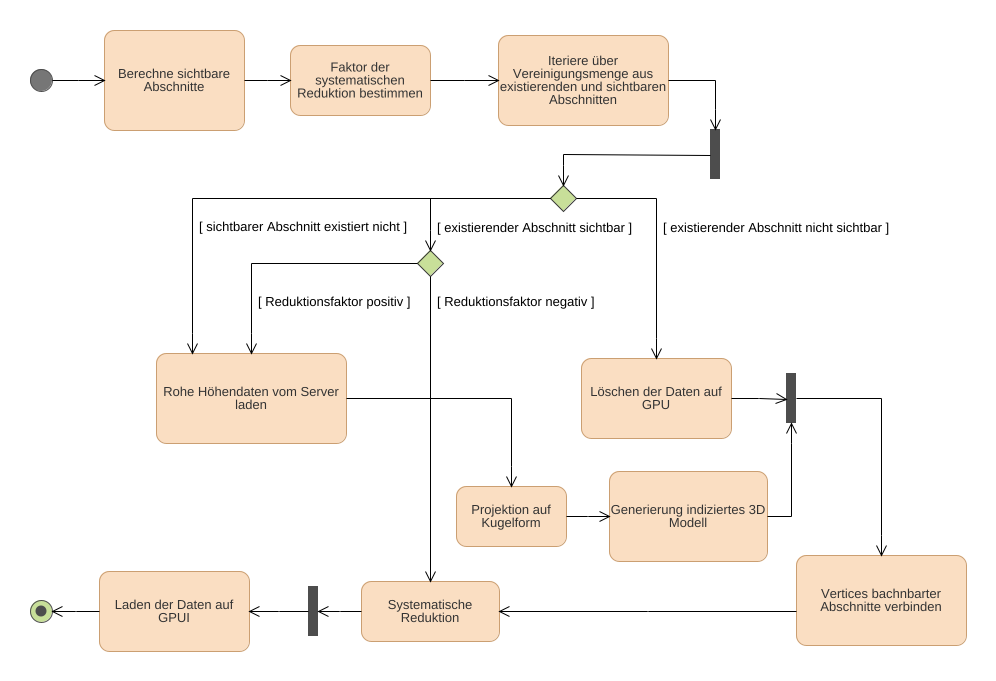
\includegraphics[width=\textwidth,keepaspectratio]{worldBuildingActivity.png}
  \caption{Aktivitätsdiagramm für die Erstellung der Welt auf Client-Seite}
  \label{worldBuildingActivity}
\end{figure}

Als erstes muss eine Liste aller sichtbaren Abschnitte angelegt werden. Dabei kommt das beschriebene frustum- und occlusion culling zur Anwendung. Da eine verlustfreie Reduktion der Datenmenge nicht ausreicht, muss eine systematische Reduktion stattfinden. Wie der Faktor schlussendlich berechnet wird, muss noch evaluiert werden, allerdings muss er von der Anzahl der sichtbaren Abschnitte abhängen und die Datenmenge auf einem möglichst konstanten Niveau halten. Als nächstes muss über die Vereinigungsmenge aller aktuell existierender und sichtbarer Abschnitte iteriert werden. Sollte der Abschnitt aktuell existieren, aber nicht mehr sichtbar sein, so muss er entladen werden. Hierbei ist darauf zu achten, auch die Ressourcen auf GPU Seite frei zu stellen, da dies natürlich nicht durch die automatische garbage collection auf JavaScript Seite abgedeckt ist. Sollte der Abschnitt aktuell existieren und auch weiterhin sichtbar sein, so muss geschaut werden, ob der Abschnitt aktuell den gleichen Reduktionsfaktor besitzt wie der berechnete. Ist dies der Fall, muss an dem Abschnitt nichts verändert werden. Sollte er größer sein, als der aktuelle Faktor, dann kann die Reduktion auf Client-Seite stattfinden, da nur eine eine bestimmte Anzahl an Vertices entfernt werden muss. Sollte er jedoch kleiner sein, so müssen die Daten erneut vom Server angefragt werden, da die Rohdaten natürlich nicht mit dem Modell gespeichert werden. Auch hierbei muss darauf geachtet werden, die aktuellen Daten zu löschen, sobald der neue Abschnitt vollständig geladen wurde. Hier muss geschaut werden, dass keine Ladeartefakte beim Tauschen des Abschnitts auftreten. Der letzte Fall in der Ladeschleife ist, dass ein sichtbarer Abschnitt nicht existiert. Hier muss dann wie beschrieben als erstes der Server nach den Daten gefragt werden. Da Netzwerkoperationen in der Regel immer relativ lange dauern, ist hier eine Parallelisierung geplant. Dies ist möglich, da in den nachfolgenden Aktionen keine Interaktion mit OpenGL notwendig ist. Als nächstes müssen die Daten in eine Kugelform projiziert werden, sollte dies vom Benutzer gewünscht werden. Auch muss aus den 1D Höhendaten jetzt ein vollständig indiziertes 3D Modell erzeugt werden. synchro end, problem der benachbarten chunks


Ein weiteres Problem, was durch die Benutzung von chunks auftritt, ist das TODO [inklusive Bild von nicht verbundenen chunks]

% Insert Komponentendiagramm und/oder Klassendiagramm

\section{User Interface}
% Einführungssatz zu mock up
% wichtig, das grundlegende Konzept zu planen und nicht jedes Detail, es ist nicht klar welche der fakultativen Anforderungen umgesetzt werden können

\begin{figure}[H]
  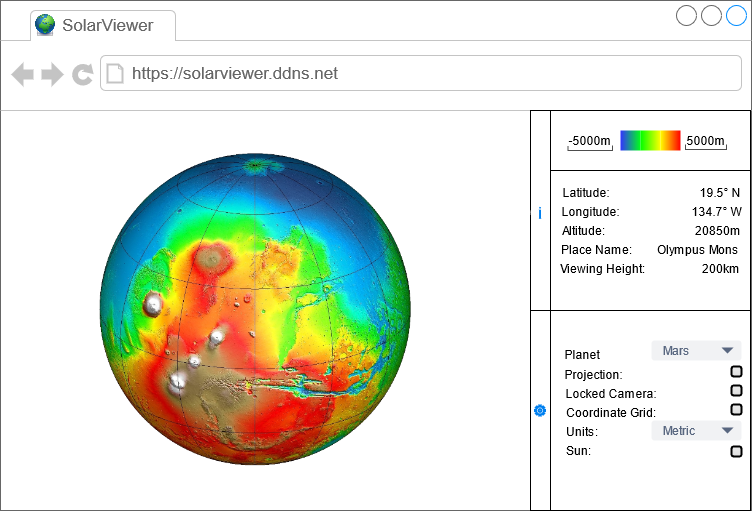
\includegraphics[width=\textwidth,keepaspectratio]{mockUp.png}
  \caption{Mock Up der SolarViewer Anwendung}
  \label{mockUp}
\end{figure}

Das Design orientiert grundsätzlich sich an den analysierten Visualisierungen (siehe \ref{istZustand}). Dabei soll die Visualisierung im Mittelpunk stehen und eine kleine UI die Navigation unterstützen und einige nützliche Informationen anzeigen. Das Hauptkriterium für die UI ist der Ansatz, dass sie die Visualisierung in keinster Weise beeinträchtigen darf. Der User soll selbst entscheiden können, welche Informationen er benötigt. Dies soll über ausfahrbare Panels realisiert werden, die von einer Seite der Anwendung ein- und ausgeblendet werden können. Dabei sollen die unterschiedlichen Panels unabhängig voneinander agieren können und möglichst ähnliche Arten von Informationen beinhalten. Fürs erste soll die UI daher in mindestens drei Bereiche gegliedert werden: Visualisierung, Informationen und Konfigurationen. Hier könnte eine Aufteilung in weitere Panels, potentiell auf der anderen Seite der UI, sinnvoll sein, je nachdem welche Anforderungen umgesetzt werden können. Alle Panels sollen über ein kleines, deskriptives Icon am Rand identifiziert werden können. Hier wurde sich an gängigen Icons orientiert und ein Zahnrad für die Konfiguration und das bekannte Informationsicon für den Informationsbereich entschieden. Die Panels sollen initial eingeklappt sein um dem User die Dimensionen der Buttons zum Öffnen der Panels zu vermitteln. Ein Klick auf die eigentlichen Panels soll keinen Effekt haben, um versehentliches Schließen der Panels zu verhindern.

Das Informationspanel soll als erstes eine Skala zeigen, die die verwendeten Farben einem Höhenwert zuordnet. Da dies natürlich eine zentrale Information ist, ohne die die Visualisierung nicht verstanden werden kann, wurde als Alternative überlegt, sie dauerhaft im Hauptteil anzeigen zu lassen. Damit würden dem Benutzer einige unnötige Klicks erspart werden, allerdings steht es im Widerspruch zum Kernkriterium, dass die Visualisierung nicht eingeschränkt werden darf. Bei besonders hohen Zoomstufen würde sich die Skala unweigerlich mit der Visualisierung überlagern und dies soll vermieden werden. Auch könnte der Nutzer diese Information dann nicht ausblenden, was ein Kernaspekt des Designs ist. Hier ist eine weitere Nutzer-Evaluation notwendig um dies zu bestätigen. Ein weiteres Problem ist die Schwierigkeit den Farben jetzt Höhenwerten zuzuordnen. Idealerweise muss dem Nutzer auf einen Blick klar sein, welche Farbe zu welchem Höhenwert gehört. Es ist jedoch aus Platzgründen schwer, mehrere Höhenangaben in die Skala aufzunehmen. Es wurde also entschieden, nur den minimalen und maximalen Höhenwert an den Rändern anzuzeigen. Hier muss vorausgesetzt werden, dass der Nutzer die Linearität versteht und sich die Höhenwerte zwischen den Grenzen erschließen kann. Auch dies muss im weiteren Verlauf mit Test-Nutzern evaluiert werden. Die Grenzen sollen laut den Anforderungen auch änderbar sein, daher muss dem Nutzer dies auch signalisiert werden. Hier wurde sich für ein Design ähnlich dem von Links entschieden, das zu einem Klick auf die Zahlen einladen soll.

Weitere Informationen auf dem Panel sollen die Koordinaten, die Höhenangabe und potentiell der Name des Ortes sein. Im Gegensatz zu den restlichen Informationen hängt es davon ab, auf welche Stelle der Nutzer auf dem Globus klickt. Hier wurde schon im voraus die fehlende Erklärung als Problem identifiziert. Es gibt kein Hinweis, der den Nutzer zu einem Klick auf den Globus verleitet. Sollte er als erstes das Informationspanel öffnen, so würden dort keine Informationen angezeigt werden können und der Nutzer könnte dies als Fehler werten. Auch ist unklar, was bei Klicks neben den Globus passieren sollte. Eine Möglichkeit wäre es, den Mauscursor zu einem bekannten, zu einem Klick verleitenden Cursor zu verändern, solange er sich über dem Globus befindet. Des Weiteren könnte man an Stelle von leeren Werte eine Textnachricht anzeigen, die den Nutzer zum Klick auf den Globus auffordert. Eine sehr gute Alternative nutzt die Google Earth Anwendung. Bei ihr kann man einen kleinen Marker per Drag\&Drop an eine bestimmte Stelle ziehen, was sehr intuitiv ist, aber gleichzeitig wohl auch zu komplex für diese Anwendung. Im Endeffekt wird wohl auch Zeitgründen eine Textnachricht zum Einsatz kommen müssen, auch wenn Text aus Gründen der User Experience immer vermieden werden sollte. Des Weiteren soll noch die Höhe des Betrachters über der Erdoberfläche angezeigt werden, dies erfordert allerdings keine besonderen Nutzerinteraktionen und stellt daher kein Problem dar. Eine Designentscheidung bei all diesen Werten ist die Genauigkeit der angezeigten Werte. Dies ist natürlich abhängig von der schlussendlichen Nutzung der Anwendung und kann zwischen wissenschaftlicher und privater Nutzung stark schwanken. Idealerweise sollte die Genauigkeit deshalb konfigurierbar sein. Als Standard wurde hier eine eher geringere Genauigkeit gewählt, die allerdings abhängig von dem verwendeten Wert ist. Der Werte der Betrachterhöhe sollte auf Kilometer, die Erdbodenhöhe auf Meter und die Koordinaten auf eine Nachkommastelle gerundet werden.

Das Konfigurationspanel soll als erstes eine Möglichkeit beinhalten, den angezeigten Datensatz, bzw. den Planeten, zu ändern. Auch wenn die Anwendung fürs erste nur den Mars visualisieren soll, soll der Visualisierung weiterer Planeten nichts im Wege stehen und dies muss schon bei der ursprünglichen UI Gestaltung beachtet werden. Des Weiteren soll der Nutzer die Projektion ein- und ausschalten können. Andere Alternativen nutzen hier noch komplexere Auswahlmöglichkeiten (z.B. unterschiedliche Kugelprojektion oder Projektionen der Pole), dies soll mit einer reinen Checkbox allerdings vereinfacht werden. Auch muss laut Anforderungen die Möglichkeit geschaffen werden, zwischen einer statischen und frei beweglichen Kamera zu wechseln. Ob hier ein besserer Weg gefunden werden kann, idealerweise ohne jedes Mal die Konfiguration zu öffnen, muss im Projektverlauf überlegt werden. Des Weiteren soll der Benutzer die Möglichkeit besitzen, die Einheiten der Höhenwerte zu ändern. Dabei soll zumindest die Wahl zwischen metrischen und imperialen ermöglicht werden. Falls im Projektverlauf keine weiteren Messsysteme gefunden werden können, kann dies auch als Checkbox realisiert werden. Des Weiteren sind in dem Panel weitere Optionen möglich, im konkreten Fall wurde Optionen zum ein- und ausschalten eines realistischen Beleuchtungsmodells und der Koordinatenlinien erdacht. Dies hängt natürlich stark von den schlussendlich implementierten Funktionen ab. Falls das Hinzufügen von Optionen aus Platzgründen schwierig wird, so muss das Informationspanel auf die andere Seite der Fensters verschoben werden.

Die Sprache der Anwendung soll Englisch sein, da so wieder die größere Zielgruppe erreicht werden kann. Insbesondere im akademischen Bereich und im Bereich der Raumfahrt sollte dies auch kein Problem darstellen, da hier Englischkenntnisse weit verbreitet sind. Die Wahl des Logos ist noch nicht final, es soll etwas universelles darstellen, was die Leute mit verschiedenen Planeten des Sonnensystems, nicht nur mit einem Planten, in Verbindung bringen. Fürs erste wurde dafür ein kleines Erdlogo geplant. Für die Icons soll der Anbieter FontAwesome genutzt werden. Er stellt in einer freien Lizenz über 1600 verschiedene Icons bereit, welche als CSS Datei, gehosted auf FontAwesome Servern, in die Webseite eingebunden werden. Konkrete Icons können dann über CSS Klassen definiert werden, wobei für jedes Icon auch verschiedene Variationen bereitgestellt werden (solide, leichtgewichtig, mehrfarbig, etc.). Auch die Größen lassen sich ohne Verlust der Auflösung stark variieren und die Farben sind frei wählbar.
\chapter{Implementierung}

\section{Build System}
Der Build Prozess ist ein Prozess, welcher alle Schritte beinhaltet um aus dem vorhandenen Source Code eine ausführbare Software zu erstellen. Insbesondere werden dabei benötigte Abhängigkeiten zur Verfügung gestellt und in die Software integriert, der Source Code kompiliert und alle Software Teile in einem ausführbaren Format zusammengeführt. Dieser Prozess kann sehr komplex werden und ist daher häufig fehleranfällig. Unter anderem die Kombination von mehreren Build Systemen und unterschiedlichen Programmierumgebungen wird dabei als ein Kernproblem angesehen\citep{buildSystemProblem}{buildSystemProblem}. Da sich dieses Projekt in ein Frontend und Backend mit unterschiedlichen Programmiersprachen gliedert, ist es allerdings notwendig unterschiedliche Build Systeme zu integrieren. Dies ist erforderlich, da die existierenden Systeme sich eher auf eine Umgebung spezialisieren und zum Beispiel nur Abhängigkeiten einer Programmiersprache in einem zentralen Repository anbieten (z.B. npm registry für JavaScript oder maven central für Java Anwendungen). Auch existieren bestimmte Plugins, zum Beispiel für das Transpilieren von TypeScript, nicht für alle Build Systeme. Alles in allem erhöht sich zwar die Build Komplexität und Dauer, allerdings hat es auch Vorteile. Zum einen führt es dazu, dass das Frontend vom Backend vollständig isoliert ist und die reine Frontendentwicklung ohne unnötige Abhängigkeiten und Build Prozesse ablaufen kann. Zum anderen erweitert sich dadurch auch die Auswahl an vorhanden Tools und Plugins, was die Entwicklung deutlich vereinfachen kann.

Für dieses Projekt wird Maven als System für das Backend und npm als System für das Frontend genutzt. Die Entscheidung wurde auf Grund der hohen Beliebtheit und der persönlichen Expertise mit diesen Tools getroffen. Aus reiner Systemsicht ist das Frontend ein Teil des Backends, da es für die Auslieferung des Frontends an den Nutzer verantwortlich ist. Der Build beginnt daher auch in Maven. Als erstes muss sichergestellt werden, dass npm und Node.js auf dem Rechner vorhanden sind. Für die Kommunikation mit diesen wird das frontend-maven-plugin\footnote{\url{https://github.com/eirslett/frontend-maven-plugin}} genutzt, welches sie in einem ersten Schritt in einen lokalen Ordner installiert, solange sie noch nicht vorhanden sind. Anschließend wird “npm install” aufgerufen, um alle deklarierten Abhängigkeiten aus dem Frontend zu installieren. Dazu zählt zum Beispiel Three.js oder auch der TypeScript Transpiler. Anschließend wird der Build an das Frontend übergeben, indem ein fest definiertes npm Script aufgerufen wird. Dieses führt als erstes den TypeScript Transpiler aus um die benötigten JavaScript Dateien anzulegen. Da npm eigentlich ein Build-Tool für Node.js, welches lokal in einem Server ausgeführt wird, müssen die Abhängigkeiten für die Verwendung im Browser besonders behandelt werden. Hier ist ein sogenannter Bundler erforderlich, welche alle Abhängigkeiten in einer lokalen Datei zusammenfasst, welche dann an den User ausgeliefert wird. Als erstes wurde das Tool Browserify in Betracht gezogen, was ein existierendes NodeJS-Projekt ohne Codeänderungen für den Browser vorbereitet. Es wurde sich jedoch für das Tool Webpack entschieden, hauptsächlich auf Grund des direkten Supports von JavaScript Modulen ohne weitere Abhängigkeiten. Die Nutzung eines Bundlers hat des Weiteren des Vorteil, dass der Code minifiziert wird und in einer einzigen Datei zusammengefasst wird, was ein deutlich schnelleres Laden der Webseite zur Folge hat. Im Gegenzug verliert man die Fähigkeit, den Frontend Code zu debuggen, da die Minifizierung dabei natürlich stark stört. Dies kann allerdings durch die Verwendung von Source Maps verhindert werden, die für genau diesen Zweck eine Zuweisung von minifizierten zu originalen Variablen- und Methodennamen zur Verfügung stellen. Um das Frontend jetzt per Webserver an den User auszuliefern, müssen die Dateien jetzt in einen Ordner im Java Classpath befördert werden. Wichtig dabei ist, dass nur die benötigten Dateien verschoben werden dürfen, da diese sonst über den Webserver erreichbar wären. Dies wäre insbesondere bei den diversen Konfigurationsdateien ein Sicherheitsproblem. Auch das Verschieben des node\_modules Ordner wäre ein grober Fehler, da dies zu einer relativ großen ausführbaren Datei führen würde. Anschließend geht der Build im Backend mit dem Kompilieren der Java Dateien weiter. Nachdem alle Tests automatisch durchlaufen wurden, werden dann alle Abhängigkeiten des Backends, unter anderem der Undertow Server, zu einem fertigen Artefakt (Fat JAR) zusammengeführt, welches dann auf einen Server deployed und dort ausgeführt werden kann.

\section{Visualisierung}
Für die eigentliche Visualisierung kommen Shader zum Einsatz. Dafür muss dem Shader natürlich der Höhenwert bekannt sein. Bei einer flachen Projektion lässt sich dieser aus dem Vertex ablesen (entsprechend skalierte y-Koordinate), dies ändert sich natürlich, sobald eine sphärische Projektion zum Einsatz kommt. Die einfachste Möglichkeit ist es, dem Shader den Höhenwert in Metern neben dem Vertex als weiteres Attribut zu übergeben. Da dies die theoretische maximale Speichernutzung allerdings um weitere 4 GB erhöhen würde, was einer Erhöhung um 1/3 der Gesamtmenge entspricht, wurde dieser Ansatz verworfen. Stattdessen ist effizienter, den Höhenwert aus dem Vertex zu berechnen. Da der Höhenwert immer der Abweichung von einem vordefinierten Radius entspricht (ähnlich dem Meeresspiegel auf der Erde), muss dieser Radius einfach von der Länge des Vertex abgezogen werden. Dies funktioniert allerdings nur, wenn der Mittelpunkt des Modells auch mit dem Koordinaten-Nullpunkt übereinstimmt, da nur dann die Länge des Vertex der Distanz zum Punkt auf der Oberfläche entspricht. Um dies im Vertexshader zu implementieren, müssen ihm die verwendete Projektion, der Radius und die Skalierung von GL Einheiten zu Metern bekannt sein. Diese werden als Uniform Werte übergeben, sind also nicht abhängig von der Vertex-Anzahl und spielen daher für die maximale Speichernutzung keine Rolle. Der Vertexshader berechnet also wie beschrieben die Höhe in Metern und gibt sie an den Fragmentshader weiter. Des Weiteren transformiert er wie üblich den Vertex mit der Model-Matrix (enthält die Transformationen des Modells), der View-Matrix (enthält die inversen Transformationen der Kamera) und der Projektions-Matrix (enthält die perspektivische Transformation der Kamera) um die endgültige Position des Vertex zu bestimmen.

Der Fragmentshader hat nun die Aufgabe, aus diesem Höhenwert einen Farbwert zu generieren. Eine Möglichkeit wäre es, einfach verschiedene Grenzen zu definieren und diesen Grenzen feste Farbwerte zuzuweisen. Dann kann geprüft werden, welchem Bereich der Höhenwert entspricht und der endgültige Farbwert entspricht dann einer Variation des Farbwerts des Bereichs. Da dies allerdings mehrere Verzweigungen (conditionals) zur Prüfung der Grenzen erfordert und dies in der Shaderentwicklung vermieden werden sollte\footnote{siehe \cite{shaderDev}, Kapitel 14, Abschnitt Avoid Dynamic Branching, S. 273}, wurde eine bessere Lösung gesucht. Insbesondere, da es sich um das sogenannte dynamic branching handelt, da da die Bedingung abhängig vom Höhenwert ist, welcher natürlich pro Vertex anders ist. Des Weiteren wurde auf Grund der Datenmenge die kritischste Stelle der Performance (bottleneck) eher auf GPU Seite angesehen, sodass hier dringender auf der Performance geachtet werden sollte. Schlussendlich wurde der Fakt genutzt, das der Hue-Wert im HSV-Farbraum eine relativ lineare Verteilung verschiedener Farben enthält und so gut als Farbskala genutzt werden kann. Da die Ausgabe des Shaders allerdings im RGBA-Format erfolgen muss, ist hier eine Umwandlung des HSV Werten in diesen Farbraum erforderlich. Es wird also der Prozentwert des aktuellen Höhenwerts abhängig von vom Nutzer definierten Grenzen berechnet und diesem Prozentwert ein Hue Wert zugeordnet. Dabei wurde der Farbraum vorher noch verkleinert und invertiert, sodass die Farben dann von einem Blau-Ton (niedrigster Wert) zu einem Rot-Ton (höchster Wert) reichen. 

\section{Kamerabewegung}
Die erste Implementierung war eine frei im Raum bewegbare Kamera, welche man mit der Tastatur steuern konnte. Als konkrete Tasten wurden zum einen die Pfeiltasten als auch die übliche Alternative WASD genutzt. Diese sind allgemein als Steuerungstasten bekannt und sollten daher keiner Erklärung bedürfen. Die Kamera bewegte sich dabei entlang des lokalen Koordinatensystems der Kamera. Dieses kann dann mit der Maus entlang der x-Achse (pitch) und y-Achse (yaw) gedreht werden. Eine Drehung um die z-Achse (roll) verkompliziert die Steuerung und wurde daher bewusst nicht implementiert. Eine Bewegung der Maus auf der x-Achse führt dabei zu einer Rotation der Kamera entlang der y-Achse und eine Bewegung auf der y-Achse zu einer Rotation entlang der x-Achse. Die Blickrichtung der Kamera folgt also effektiv der Bewegung der Maus. Dabei wurde das Drehen nur beim Gedrückthalten der Maustaste (dragging) durchgeführt, da die Kamera sich sonst natürlich bei der normalen Navigation auf der Seite bewegen würde. Das Gedrückthalten ist dabei schon weniger intuitiv, allerdings entspricht es der physischen Bewegung des Ziehens an einer Seite des Globus in der realen Welt. Hier ist allerdings eine genauere Evaluation der Steuerung notwendig um eine gute User-Experience zu gewährleisten.

Wichtig bei der Implementierung ist, dass die Geschwindigkeit der Bewegung nicht von der Geschwindigkeit des Browser abhängen darf. Daher müssen alle Vektoren, welche eine Bewegung darstellen, mit der Zeit multipliziert werden, die seit dem letzten Aufruf der Bewegung vergangen ist. Nur so wird in einem bestimmten Zeitabschnitt immer die gleiche Länge zurückgelegt. Ein weiterer Aspekt ist, dass das Gedrückthalten einer Taste natürlich zu einer kontinuierlichen Bewegung führen soll. Um dies zu erkennen kann zum einen das keydown-Event des Browser genutzt werden, welches auch gesendet wird, solange die Taste gedrückt bleibt. Allerdings ist dabei eine spürbare Verzögerung zwischen erstem und nachfolgenden Events vorhanden, sodass die Bewegung initial ziemlich ruckartig erfolgt. Auch ist die Geschwindigkeit, mit der die Events gesendet werden, nicht definiert und kann so zu sehr ruckartigen Bewegungen führen, sollte die Rate weit unter der Bildwiederholrate des Monitors liegen. Stattdessen werden die Kameras in der Render-Schleife, begrenzt durch die Bildwiederholungsrate (vSync), so lange in der gleichen Konfiguration geupdated, bis ein entsprechendes keyup-Event der gleichen Taste registriert wurde.

Die zweite Implementierung ist die stationäre Kamera, welche sich um den Globus in einem festen Abstand bewegt. Auch hier wurde die Rotation durch das Dragging der Maus implementiert. Da beide Kameras die selben Steuerungsmöglichkeiten besitzen sollte dies für den User schnell verständlich sein. Der Abstand zum Globus kann dabei mit dem Mausrad verändert werden, was auch sehr intuitiv sein sollte. Beim ersten Ansatz der Implementierung wurde die Kamera zum Rotierungspunkt (Pivot) bewegt, um den entsprechenden Winkel rotiert und anschließend im lokalen Koordinatensystem entlang des ursprünglichen Bewegungsvektors zurück bewegt. Ein wesentlich einfacher und genauerer Ansatz wurde dann in der Form des Scene-Graphs der THREE Bibliothek gefunden. Dabei wird eine Hierarchie an Objekten in Form einer Baumstruktur definiert und alle Transformationen eines Objektes werden automatisch an dessen Kinder weitergegeben. Wenn jetzt die Kamera als Kind des Pivot definiert wird, dann kann dieser normal rotiert werden und die Kamera rotiert automatisch im selben Winkel und Abstand mit. Für das Zoomen wurde das wheel-Event genutzt, welches Informationen darüber enthält, wie stark das Mausrad rotiert wurde. Hier gibt es die unterschiedlichen Einheiten Pixel, Zeilen und Seiten, welche auf die Navigation einer normaleren Seite mit Text ausgelegt sind. In konkreten Fall wurde nur die Scrollrichtung ermittelt und die Kamera mit einem festen Betrag entlang der lokalen z-Achse verschoben. Zusätzlich wurden minimale und maximale Abstände definiert und von der Implementation beachtet, damit die Kamera nicht über den Nullpunkt hinaus scrollt und somit effektiv die Scrollrichtung ändert.

Beide Implementationen updaten nach Erkennen jeglichen User-Inputs die View-Matrix und senden dann ein spezielles Event aus, dass den Ladeprozess\ref{dataLoading} in Gang setzt. Hier fiel auch ohne viel Testen auf, dass ein Anstoßen des Ladeprozesses bei jeder Interaktion performancetechnisch nicht durchführbar ist, da der Browser die Events in einer viel zu hohen Frequenz ausliefert. Es musste also eine Art Limitierung implementiert werden, die die Events auf eine maximale Rate beschränkt. Wichtig dabei war der Punkt, dass auch das letzte Event immer zugestellt werden musste. Es konnte also nicht einfach ein Zähler hochgezählt werden, der die vergangene Zeit inkrementiert und beim Erreichen des Limits das Events weiter propagiert, da natürlich jedes Event das potentiell Letzte sein könnte. Stattdessen wurde die setTimeout-Funktion des Browsers genutzt, welche das Event am Ende der Wartezeit propagiert. Nachfolgende Events löschen dann den jeweils aktuellen Timeout und stellen sich selbst als Wartender in die virtuelle Warteschlange. Die Limitierung wurde im konkreten Fall auf 1 Event pro Sekunde gesetzt, was ein guter Kompromiss zwischen Performance und ausreichend dynamischem Ladens der Welt darstellt. Dieser feste Wert sollte idealerweise während der Laufzeit an die aktuelle Hardware angepasst werden um User Experience auf guter Hardware noch zu verbessern. Da dies jedoch nur eine fakultative Anwendung darstellt und das Finetuning zu viel Zeit in Anspruch genommen hätte, wurde es nicht implementiert.

\section{Daten-Ladeprozess}\label{dataLoading}
Nachdem der Datenladeprozess in Gang gesetzt wurde, werden als erstes alle Abschnitte berechnet, die sichtbar sind. Dafür muss als erstes das Frustum für die aktuelle Kamerasicht initialisiert werden. Für jeden potentiellen Abschnitt wird jetzt geprüft, ob dieser auch nur ansatzweise das Frustum schneidet. Auch wenn nur ein einzelner Vertex den Sichtbereich schneidet muss der gesamte Abschnitt gerendert werden, da ein Abschnitt nicht weiter aufgeteilt werden kann. Da diese Schnittberechnung für ein Modell mit insgesamt über einer Milliarde Vertices natürlich nicht durchführbar sind, wurden Hüllobjekte genutzt, welche einmalig für den gesamten Globus angelegt wurden. Dabei wird jeder Abschnitt durch ein Rechteck definiert, wodurch nicht wirklich von einem Hüllobjekt gesprochen werden kann. Die Höhenwerte des Abschnitts werden dabei ignoriert, da die Höhe im Vergleich zur Ausbreitung eines Abschnitts verschwindend gering ist. Auch die Krümmung eines Abschnitts konnte dabei nicht beachtet werden, da das Hüllobjekt natürlich nur 4 Vertices besitzt. Das Rechteckt orientiert sich an den originalen Maßen des Abschnitts und besitzt die selbe Position und Orientierung, sodass ein relativ gutes Modell des eigentlichen Planeten entsteht. Es ist jedoch nicht perfekt und es kann vorkommen, dass Abschnitte am Rand des Globus nicht angezeigt werden, obwohl sie auf Grund der Krümmung und/oder besonders hoher Oberflächenstrukturen angezeigt werden müssten. Solange eine Projektion stattgefunden hatte, muss jetzt natürlich noch das occlusion culling durchgeführt werden, da Abschnitte am anderen Ende des Globus verdeckt sein könnten und so nicht gezeichnet werden brauchen. Ein erster Implementationsversuch berechnete die Distanz von der Kamera zum nächstliegenden Abschnitt in Blickrichtung der Kamera. Danach wurde diese Distanz mit den Distanzen zu allen anderen Abschnitten verglichen. Sollte die Distanz zu einem Abschnitt größer sein als die Distanz zum nächstliegenden plus dem Radius des Globus, so muss dieser zwingend auf der anderen Seite des Globus sein. Das funktionierte bei einem großen Abstand relativ gut, allerdings wurde nicht bedacht, dass dieses Prinzip nur bei einer frontalen Ansicht funktioniert. Sollte die Blickrichtung den Globus seitlich schneiden, so ist eine viel geringere Distanz als der Radius notwendig um Abschnitte auszuschließen. So wurden zu viele Abschnitte geladen, was einen deutlichen Einfluss auf die Performance hatte. Der zweite Ansatz nutze das Prinzip des Raytracings, bei dem ein Strahl zum Abschnitt gesendet wird und die Abschnitte berechnet werden, die diesen Strahl schneiden. Alle gefunden Abschnitte müssen dann entlang der Blickrichtung an Hand ihrer Distanz sortiert werden und sollte ein Abschnitt vor dem zu testenden Abschnitt liegen, so ist er nicht sichtbar. Da hier natürlich wieder Schnittberechnungen für jeden Abschnitt gegen jeden anderen Abschnitt, also mit einer quadratischen Komplexität, durchgeführt werden müssten, muss auch hier die Performance beachtet werden. Neben dem direkten Ausschluss des Sendens eines Strahl zu jedem Vertex eines Abschnitts wurde versucht, ein Strahl zu jedem Eckpunk des Hüllobjekts zu senden. Allerdings reichte dies nicht aus, um die geforderte Framerate zu erreichen, sodass hier nur ein Strahl zum Mittelpunkt des Abschnitts gesendet wurde. Dies führt allerdings noch stärker zu nicht ladenden Abschnitten am Rand des Globus, falls die Hälfte des Abschnitts theoretisch noch sichtbar wäre. In zukünftigen Projekten sollte hier mehr Aufwand betrieben werden, um verdeckte Abschnitte besser zu bestimmen.

Nachdem die Liste mit den zu ladenden Abschnitten angelegt war, musste ein Reduktionsfaktor berechnet werden. Dieser muss in der Lage sein, die Dimensionen eines Abschnitts gleichmäßig teilen zu können. Dies ist notwendig, da sie an den Kanten definiert sein müssen um sich mit benachbarten Abschnitten verbinden zu können. Des Weiteren muss er linear von der Anzahl der Abschnitte abhängen, da mit steigender Anzahl natürlich auch die Datenmenge steigt. Auch muss er bei hohen Zoomstufen, also bei einer geringen Abschnittsanzahl, möglichst gering sein, da die Auflösung vom Nutzer hier wahrgenommen werden kann. Schlussendlich sollt dieser Faktor sich nicht allzu oft ändern, da jede Änderung ein potentielles Neuladen der Abschnitte in Gang setzen kann. Konkret wurde die Anzahl der Abschnitte auf die nächste Zweierpotenz abgerundet, da so eine geringe Schwankung bei einer höheren Anzahl auftritt, was der Nutzer nicht unterschieden kann. Bei einer geringen Anzahl von Abschnitten steigt die Wechselfrequenz an, was sehr vorteilhaft ist. Auch sind Zweierpotenzen Teiler der Dimensionen der Abschnitte. Nachdem der Faktor berechnet wurde, wird über alle aktuellen Abschnitte iteriert und alle nicht mehr wahrgenommenen Abschnitte werden aus einer internen Datenstruktur als auch aus dem Grafikspeicher entfernt. Anschließend werden alle sichtbaren Abschnitte geladen, falls diese noch nicht existieren oder ursprünglich einen anderen Reduktionsfaktor aufweisen.

Es wurde bereits kurz das Problem der nicht verbundenen Abschnitte angesprochen. Dies tritt zum einen auf, da unterschiedliche Abschnitte keine Vertices mit den umliegenden Abschnitten teilen (siehe Abbildung \ref{chunkSeparation}). Zum anderen tritt es in der sphärischen Projektion auf, wenn die Ränder des Datensatzes am anderen Ende der Kugel wieder auf den Anfang treffen (siehe Abbildung \ref{mapEndSeparation}). Hier wurde erst überlegt, auf Client Seite die Vertices der Ränder jeweils benachbarter Abschnitte in den eigenen Abschnitt zu kopieren. Da ein Auslesen von Vertexdaten aus dem Grafikspeicher (Vertices sollen möglichst nicht im RAM gehalten werden) jedoch aufwendig ist und die Daten bereits im Backend vorliegen, wurde hier entschieden einfach das Anfrageraster zu vergrößern, sodass sich die Abschnitte effektiv überlappen. Ein Problem war dabei, dass die ImageIO-API, welche im Backend genutzt wurde um Ausschnitte aus den Originaldaten auszulesen, nicht zur Lösung des Problems des Verbindens der Ränder des Datensatzes geeignet war. Man musste in x-Richtung effektiv wieder zum Anfang des Datensatzes springen, was eine weitere Anfrage und ein mühseliges Kopieren einer weiteren Spalte in eine reihenbasierte Datenstruktur erforderte. In y-Richtung müssen die Werte allerdings die gegenüberliegenden Werte in der Kugelprojektion weiterführen, wobei jeder Wert y abhängig von der aktuellen Position x durch die folgende Formel erlangt werden könnte: \[y = x\]



\begin{figure}[!tbp] 
  \centering
  \begin{minipage}[b]{0.4\textwidth}
    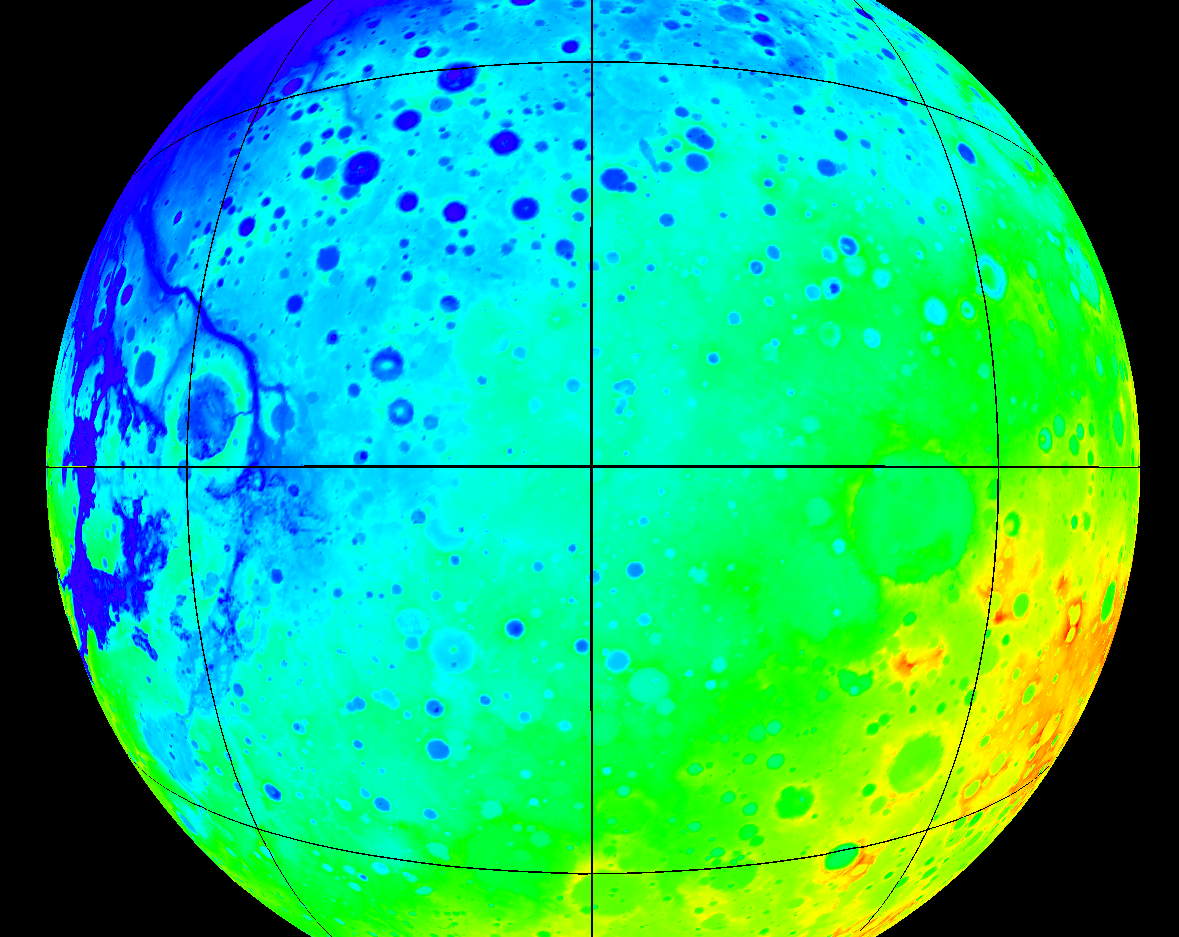
\includegraphics[width=\textwidth]{chunkSeparation.png}
    \caption{Abstands-Artefakte an den Rändern von Abschnitten}
    \label{chunkSeparation}
  \end{minipage}
  \hfill
  \begin{minipage}[b]{0.4\textwidth}
    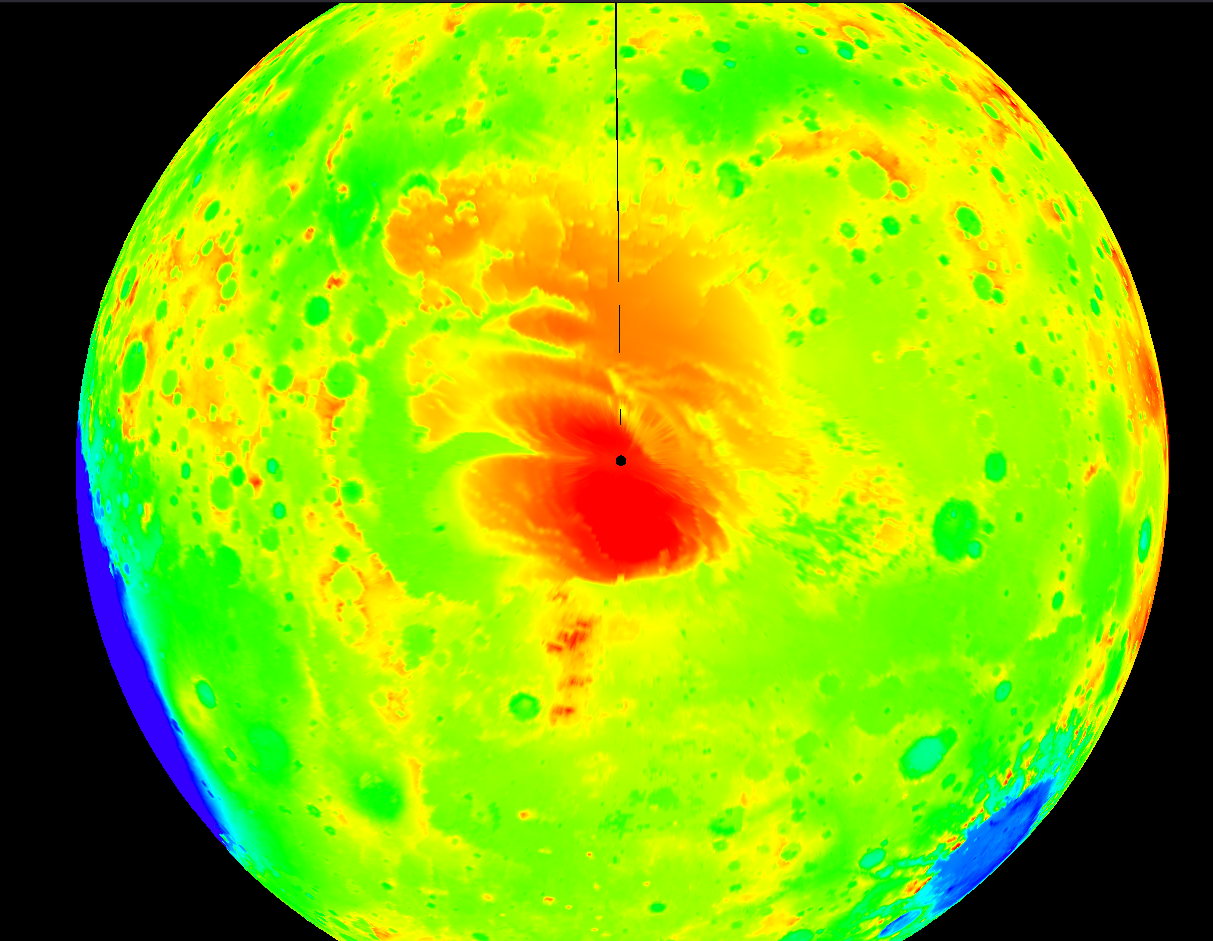
\includegraphics[width=\textwidth]{mapEndSeparation.png}
    \caption{Abstands-Artefakte an den Rändern des Datensatzes in x- und y-Richtung}
    \label{mapEndSeparation}
  \end{minipage}
\end{figure}

\section{User Interface}

% insert screenshot der fertigen Anwendung
% beschreibe hier vor allem, wie es alles zusammenhängt, also zum Beispiel die Inputs dann die Uniform Werte anpassen müssen oder zum Beispiel das Kamerascript ändern, was von der HRender-Schleife geupdated wird (wichtig dabei ist es, die jeweiligen Kamera-Scripte zu deaktivieren, da sie immer noch Nutzervenets erhalten)

\section{Tests}
Beim Testen der Anwendung hat dieses Projekt das gleiche Probleme aller Grafikprojekte: die Visualisierung kann ohne weiteres nicht automatisch getestet werden. Die Ausgabe auf dem Bildschirm ist zu komplex um daraus Testfälle zu definieren. Auch existieren zu viele Parameter, die das schlussendliche Ergebnis beeinflussen. Und natürlich könnte man Teile des Prozessen testen, zum Beispiel die Erstellung des 3D-Modells auf CPU Seite, allerdings ist es auch dort schwer erwartbare Testfälle zu definieren. Es ist einfach nicht definierbar, wie der Vertex auszusehen hat, der dem n-ten Höhenwert entspricht. Auch die Frage ob Formeln richtig implementiert wurden, lässt sich nur durch die Implementation der Formel im Test testen, was dem Sinn eines Tests widerspricht. Stattdessen wurden in diesem Projekt im Frontend viele manuelle Tests durchgeführt. Zum einen wurde die Visualisierung mit anderen Visualisierungen verglichen. Dabei reichte oft schon ein 2D Bild eines Referenzbildes einer verlässlichen Quelle, im konkreten Fall eine ähnlich eingefärbte Karte des gleichen Datensatzes vom JPL. Außerdem wurde mit Hilfe des Koordinaten und Höhenangaben Features bekannte geographische Features wie den Olympus Mons oder Hellas Planitia gegengeprüft. Da diese Features die Werte an Hand des Vertex berechnen und nicht die originalen Höhenwerte referenzieren, ist es eine recht gute Möglichkeit. Es ist sehr unwahrscheinlich, dass in beiden Implementationen Fehler enthalten sind, die sich gegenseitig aufheben zu richtigen Testresultaten führen. Ansonsten wurde zum Beispiel manuell sichergestellt, dass keine Lücken in der Visualisierung zu sehen sind oder dass die Panels wie geplant aus- und einklappen können. Auch die unterschiedlichen Kamerabewegungen wurden manuell überprüft. Nur bei der Konfiguration der maximalen und minimalen Höhe für die Interpolation wäre ein automatischer Test für das Verhalten bei falschen Benutzereingaben denkbar gewesen. 

Im Backend dagegen wurde jede öffentliche Methode zumindest mit einem Testfall abgedeckt. Relativ viel Aufwand wurde beim Testen der Redundanzentfernung betrieben. Hier wurde ein unbekannter Algorithmus getestet, der insbesondere keine optimale Lösung finden kann. Dadurch wurden viele Testfälle definiert, die prüfen, ob sehr einfache Optimierungsfälle, wie zum Beispiel die Überprüfung aller Alternativen bei nachfolgenden linearen Abhängigkeiten, eingehalten wurden. Auch Edge Cases konnten hier schön abgedeckt werden, zum Beispiel Fälle von Redundanzen die am Rand eines Abschnitts liegen oder bei denen redundante Teilraster nebeneinander liegen. Für den Endpoint wurden Tests geschrieben, die sicherstellen, dass die Redundanzentfernung korrekt ausgeführt wird und das alle Parameter (Position, Dimension, Reduktionsfaktor) korrekt behandelt werden.

\chapter{Evaluation}

\section{User Experience}
Der erste Punkt, der evaluiert werden muss, ist, ob die Anwendung in ihrer jetzigen Form von der Zielgruppe verstanden wird. Dabei muss zum einen die Bedienung der Anwendung als Ganzes überprüft werden. Dazu zählt zum einen, dass das User Interface ohne Erklärungen bedient werden kann und bestimmte Aufgaben aus dem Use Case erfüllt werden können. Zum anderen muss die Visualisierung korrekt interpretiert werden können. Hier ist zum Beispiel zu prüfen, ob der Benutzer von Anfang an die Farben einzelnen Höhenwerten zuordnen kann. Auch die Kamerasteuerung ist ein wichtiger Aspekt, der hier überprüft werden muss. Hier sollte geprüft werden, welche der beiden Kameraimplementationen vom User bevorzugt wurden und ob beide Implementationen zur Erfüllung des Use Case nützlich waren. Auch bestimmte Details wie das Dragging der Maus zum Umsehen wurde während des Projekts als potentiell erklärungsbedürftig eingestuft, muss hier also überprüft werden. Neben der Intuitivität muss auch überprüft werden, wie gut der User mit der Kamera zurecht kommt. Hier ist wichtig, dass der Nutzer sowohl bei hohen Zoomstufen als auch aus großer Entfernung flüssig bestimmte Orte an navigieren kann. Hier ist die Sorge, dass die Geschwindigkeit der Kamera bei einer geringen Distanz zu groß ist, insbesondere bei der rotierenden Kamera. Mit der frei bewegbaren Kamera ist die Idee, dass sich bestimmte Punkte leichter erreichen lassen, da hier die laterale Bewegungen (Steuerung der Blickrichtung) linear abhängig von der Mausbewegung ist, welche in der Regel sehr präzise sein kann. Schlussendlich muss überprüft werden, welche Auswirkungen die Techniken zur Datenreduktion auf die User Experience haben. Dazu soll geprüft werden, in weit die Tester das Nachladen von Abschnitten wahrnehmen, bzw. wie störend sie es empfinden. Idealerweise sollten natürlich keine Ladeartefakte zu sehen sein, dies kann auf Grund eigener Tests jedoch ausgeschlossen werden. Außerdem ist zu ermitteln, ob die Tester die dynamischen Auflösungsanpassungen wahrnehmen können.

Die Durchführung der Evaluation gestaltete sich auf Grund der aktuellen Covid-19 Pandemie als sehr schwierig. Insgesamt konnten nur vier Personen aus der Zielgruppe gefunden werden, die die Anwendung testeten. Dies reicht natürlich nicht aus, um eine repräsentative Meinung dazu zu erhalten, allerdings reichte es, um einige Probleme mit der Anwendung aufzudecken. Als erstes wurde die Anwendung unter einer öffentlichen Domain gehosted, sodass der Zugang kein Spezialwissen über den Build-Prozess benötigte. Anschließend wurde ein Fragebogen übermittelt, der die oben genannten Punkte abdeckte. Hier wurde als erstes ein Use Case definiert, den die Benutzer abzuarbeiten hatten. Konkret sollte mit Hilfe aller Features der höchste Punkt auf dem Mars gefunden werden. Die Idee dahinter war, dass der Nutzer an Hand der Farben relativ schnell einen hohen Punkt findet, den Höhenwert an Hand des Klicks auf den Globus ermittelt und im Konfigurationsmenü daraufhin die Skala so anpasst, dass kleinere Werte nicht mehr beachtet werden. Dieser Prozess, welcher leicht an eine Binärsuche erinnert, sollte dann iterativ wiederholt werden. Die Benutzer bekamen dabei natürlich keine Erklärungen und die Erwartung war auf Grund eigener Tests um die zwei oder drei Iterationen. Dieser Use Case involviert die Zusammenarbeit verschiedener Features und testet, ob der Nutzer die Visualisierung einordnen kann. Insbesondere wurde damit auch der kritische Punkt abgedeckt, dass die Erklärung des Höhenmessfeatures nirgendwo beschrieben und seine Indikation während des Projekts als zweifelhaft eingestuft wurde. Die Benutzer nahmen dann eine Bewertung auf dem Fragebogen vor, wobei hier oftmals eine Skala genutzt wurde um festzustellen, wie gut der Tester dies erfüllen konnte oder wie gut er mit der jeweiligen Interaktion zurecht kam.

Den gestellten Use Case konnten alle Tester relativ gut erfüllen. Hier ist festzuhalten, dass die Genauigkeit relativ stark schwankte und einige Tester sich dabei mehr oder weniger Mühe gegeben hatten, den Punkt auch wirklich genau zu finden. Alle fanden jedoch die ungefähre Umgebung und einen recht hohen Höhenwert. Auch ist wichtig, dass alle Tester zumindest einmal die Skala anpassten, da sie feststellten, dass die Skala in ihrer Standardkonfiguration nicht ausreichte um den höchsten Punkt zu finden. Alle Tester fanden ohne Erklärung heraus, wie die Position und die Höhe eines Punktes ermittelt werden kann und wo dies angezeigt wird. Hier war die Sorge also unbegründet und es muss keine weitere Verbesserung vorgenommen werden. Für die Erfüllung des Use Case nutzen alle Tester die gleiche rotierende Standardkamera. Alle konnten diese intuitiv steuern und es gab keine Erklärungsnotwendigkeit beim Dragging. Sie bewerteten die Steuerung hier alle mit der höchsten Punktzahl. Die sich frei bewegende Kamera dagegen wurde weniger gut bewertet und drei der Tester konnten damit sehr schlecht umgehen. Hier wurde vor allem kritisiert, dass es sehr lange dauert, zur anderen Seite des Globus zu gelangen und dass ein Ändern der des Betrachterwinkels auf der y-Achse (Inklanation) sehr schwierig ist. Hier müsste der Nutzer sein Blickwinkel strikt nach oben richten, sich dann leicht vorwärts bewegen und dann wieder den original Blickwinkel einnehmen, ohne das dabei die Position auf der x- oder z-Achse verändert wurde. Hier hätte eine weitere Taste integriert werden können, mit dem man die Kamera entlang der Blickrichtung hoch oder runter bewegen könnte. Im Gegensatz zu den Steuerungstasten WASD oder den Pfeiltasten sind jedoch dafür keine Tasten bekannt, sodass dieses Feature wahrscheinlich nicht ohne Erklärung wahrgenommen wäre. Alle Tester waren schlussendlich der Meinung, dass die frei bewegliche Kamera, zumindest in der Kugelprojektion, nicht hilfreich ist. Die Ansicht ohne Projektion wurde von allen Testern als neutral beurteilt und viele sahen dafür keinen echten Grund. Die Ansicht als Globus wurde jedoch von allen Testern bevorzugt. Die Unterteilung in Abschnitte wurde wie erwartet von allen Testern wahrgenommen und als störend empfunden, sodass hier deutliche Verbesserungen vorgenommen werden müssen. Die Anpassung der Auflösung zur Laufzeit wurde allerdings nicht wahrgenommen, das Tauschen von existierenden Abschnitten zur Laufzeit war also ein Erfolg.

Des Weiteren konnten die Tester allgemeine Kommentare und Verbesserungsvorschläge über die Anwendung abgeben. Hier wurde zum einen mehrmals angemerkt, dass die 3D Darstellung der Oberfläche schlecht zur Geltung kommt. Dies ist natürlich zutreffend, da das Verhältnis von Höhen zum Durchmesser des Planeten natürlich absolut gering ist. Auch die Farben haben hier nicht ausgereicht, um, besonders bei hohen Zoomstufen, einen Höhenunterschied zu simulieren. Für zukünftige Projekte wurde hier geplant einen Konfigurationsparameter hinzuzufügen, der Höhenwerte zusätzlich verstärken kann. So ein Parameter war rückblickend betrachtet auch in einer der analysierten Alternativen zu finden, sodass dies ein Problem darstellt, was bereits bekannt war. Hier muss dann natürlich immer überlegt werden, inwieweit man die Darstellung von einer realistischen Darstellung entfernen will, ein Punkt, der sehr stark vom späteren Use Case abhängt. Außerdem bemängelten die Hälfte der Tester, dass die Farbskala nicht dauerhaft zu sehen war und dass ein dauerhaftes Ausklappen des Informationspanels störend wäre. Hier hätte also eine Trennung stattfinden können, wobei die andere Hälfte dies natürlich als nicht störend empfunden hatte.

\section{Profiling}
Nachdem die Anwendung funktional auf einem akzeptablen Stand war, musste verifiziert werden, dass dies auch für die Performance zutraf. Insbesondere, da diese, auf Grund der Datenmenge, natürlich besonders im Vordergrund steht. Da die Performance natürlich von Testern nicht in ausreichendem Maße ermittelt werden kann, konnte die Performance nur in Eigenanalyse auf einem Satz Hardware durchgeführt werden. Dies ist natürlich nicht ausreichend um die Performance für verschiedene Performanceklassen zu bestimmen. Dies führt auch dazu, dass die Anpassung der Visualisierung an verschiedenste Hardwarebedingungen, wie in den nicht-funktionalen Anforderungen (siehe \ref{nichtFunktional}) beschrieben, nicht getestet werden kann. Konkret dafür genutzt wurde ein Rechner mit einer GeForce GTX 970 Grafikkarte mit 4 GB VRAM, einer Intel i7-4790K 4 GHz CPU und 16 GB DDR3 RAM. Die Anwendung wurde bei allen Tests in Google Chrome 94 getestet. Die maximale Downloadgeschwindigkeit beträgt 100 Mbit/s auf einer DSL Leitung. Alle hier ermittelten Messwerte sind der Durchschnitt aus mehreren Messungen, wobei der Browsercache natürlich nach jedem Durchlauf geleert wurde. Ein Problem beim Profilen der GPU ist, dass es nahezu unmöglich ist, von außen nur die Performancedaten der eigenen Anwendung zu ermitteln. Auf CPU Seite existieren dagegen Threads, welche man unabhängig von den anderen Threads betrachten kann. Viele GPU Profiling Tools nutzen daher das Konzept der Instrumentierung, bei dem der Code mit Analyse Code erweitert wird. Das konnte auf Grund von Zeitgründen bei diesem Projekt nicht durchgeführt werden und im folgenden sind die Daten der GPU durch andere Anwendungen leicht verfälscht.

Die Punkte, welche hier überprüft werden müssen, sind teilweise in den nicht-funktionalen Anforderungen definiert und sind vor allem die Auslastung von Grafik- und Arbeitsspeicher. Diese darf selbst bei vielfachen Benutzeraktionen die Grenze von 4 GB bzw. 8 GB nicht überschreiben. Außerdem ist die erreichte Anzahl an Frames pro Sekunde (FPS) zu ermitteln, womit überprüft werden kann, wie gut der Spagat aus Performance und User Experience gelungen ist. Auch die Auslastung von CPU und GPU zu allen Zeiten ist zwar nicht definiert, sollte jedoch auf einem akzeptablen Maß liegen. Ein weiterer Punkt ist auch die Ladezeit bis zum vollständigen Laden aller Abschnitte in der initialen Ansicht. Dies ist der erste Eindruck eines jeden Nutzers und sollte dementsprechend relativ gut sein. 

Ein erstes Profiling mit Hilfe der Entwicklertools stellte schnell fest, dass die Anwendung weder auf CPU- noch auf GPU-Seite ausgelastet ist. Auf CPU Seite wurde während des gesamten Tests  nur 16\% der Zeit im JavaScript verbracht (siehe Abbildung \ref{cpuUsage}). Auch die Zeit in der GPU stellte mit 3.5\% einen sehr geringen Anteil dar (siehe Abbildung \ref{gpuUsage}). Dies sagt natürlich noch nichts darüber aus, wie stark der Prozessor während einzelner, spezieller Zeiten genutzt wurde. Aber auch dort kann in Abbildung \ref{overallPerformance} gesehen werden, dass nach einer vollen Auslastung beim Laden der Seite jemals wieder eine volle Auslastung erreicht wurde. Auch erreichte sie nach dem initialen laden fast dauerhaft 60 FPS (grüne Linie), was auf dieser Hardware laut den Anforderungen eigentlich zu hoch ist. Es waren zwar einzelne Einbrüche auf 30 FPS zu sehen\footnote{vSync führt hier dank des Wartens auf das nächste Refresh-Intervall zu so einem starken Abfall}, diese können jedoch nicht durch eine besonders starke GPU Auslastung zu bestimmten Frames erklärt werden.

\begin{figure}[H]
  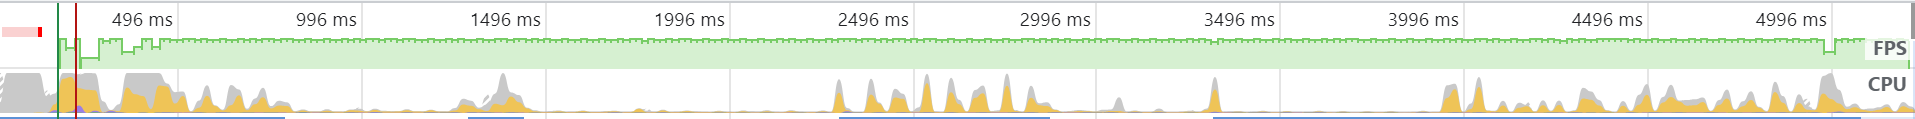
\includegraphics[width=\textwidth]{overallPerformance.png}
  \caption{CPU Auslastung und Framerate über Zeit}
  \label{overallPerformance}
\end{figure}

\begin{figure}[H]
  \begin{minipage}{0.5\textwidth}
    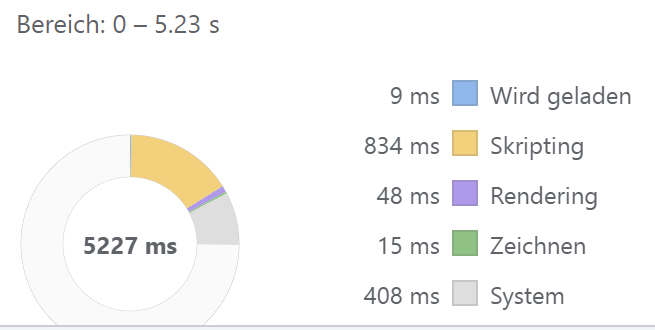
\includegraphics[width=0.95\textwidth]{cpuUsage.png}
    \caption{Totale CPU Auslastung}
    \label{cpuUsage}
  \end{minipage}
  \begin{minipage}{0.5\textwidth}
    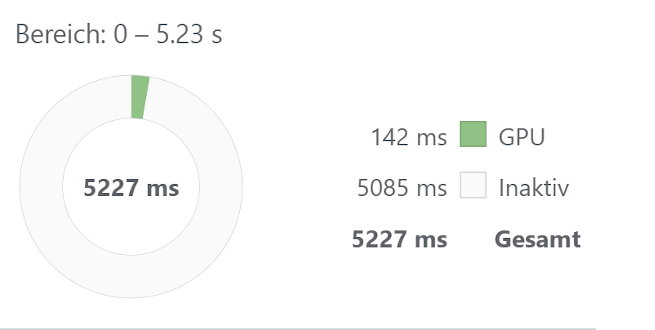
\includegraphics[width=0.95\textwidth]{gpuUsage.png}
    \caption{Totale GPU Auslastung}
    \label{gpuUsage}
  \end{minipage}
\end{figure}

Trotzdem waren bei der Benutzung der Anwendung relativ starke Lade-Artefakte zu sehen. Man konnte das Laden der einzelnen Abschnitte verfolgen und es kam zu spürbaren Verzögerungen zwischen vollständigen Ansichten. Hierzu muss natürlich gesagt werden, dass per starker Kamerabewegungen der Ladeprozess unnatürlich stark beeinflusst wurde. Es wurde sowohl das Laden von neuen Abschnitten als auch die Änderung des Details Grades stark forciert, was nicht einer normalen Nutzung entspricht. Hier wurde festgestellt, dass die Anwendung bei einer so großen Datenmenge durch das Netzwerk ausgelastet ist (siehe Abbildung \ref{requests}).

\begin{figure}[H]
  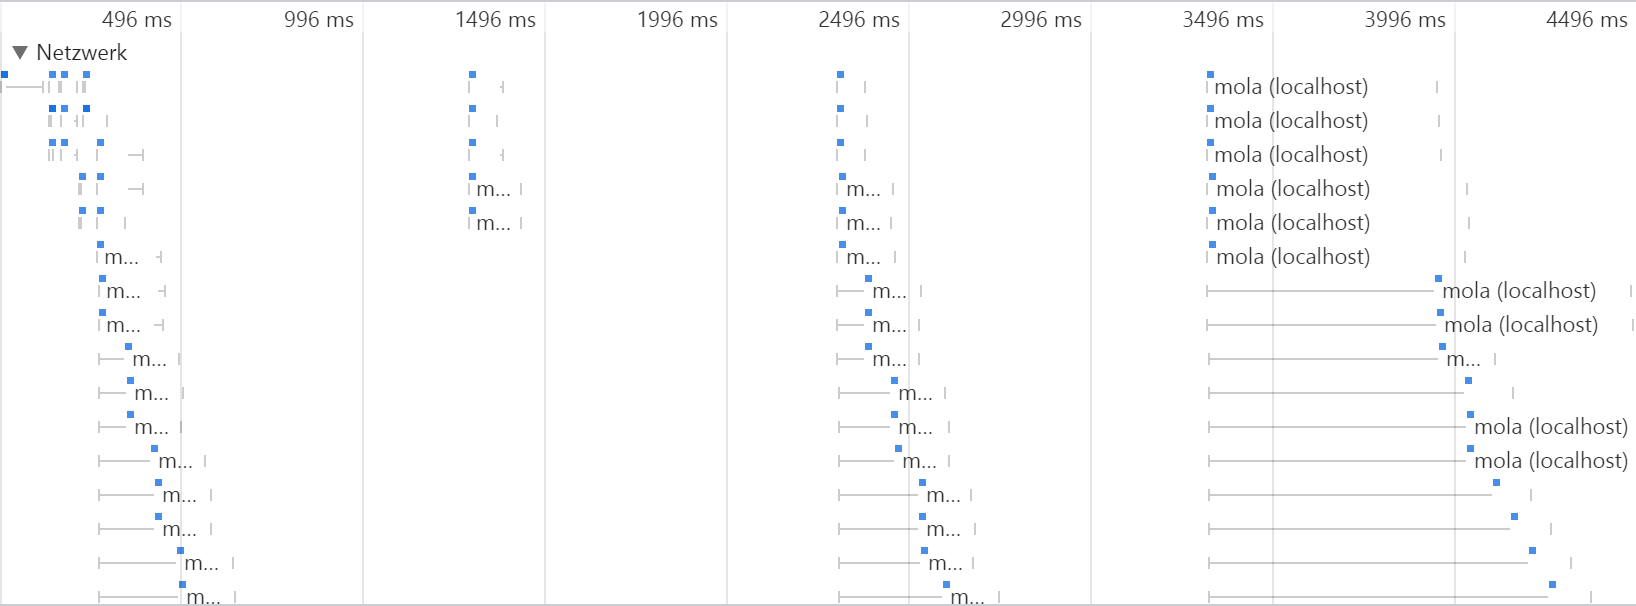
\includegraphics[width=\textwidth]{requests.png}
  \caption{Dauer der Laderequests über Zeit}
  \label{requests}
\end{figure}

Hier sind die Dauer der einzelnen Requests über die Zeit zu sehen und man kann deutlich sehen, dass diese mit der Zeit immer länger dauern. Auch lässt sich deutlich die Drosselung des Ladevorgangs auf jede Sekunde erkennen, da sich alle Requests einer Gruppe mit gleicher Anfangszeit zuordnen lassen. Am Anfang waren diese Requests mit 70 ms bis maximal 150 ms schon relativ hoch. Auch die Dauer einzelner Requests pro Vorgang wuchs an, was darauf hindeutet, dass pro Ladevorgang schneller Requests gesendet wurden, als das diese bearbeitet wurden. Noch kann man allerdings erkennen, dass eine Gruppe vollständig fertig mit Laden ist, bevor der nächste Ladezyklus beginnt. Nach einigen Sekunden steigt die Dauer der Requests dann allerdings plötzlich auf 700 ms bis maximal 1.5 s an, was nicht mehr vertretbar ist. Ab diesem Zeitpunkt überlagern sich dann auch die Ladezyklen (siehe Abbildung \ref{requestOverlap}). 

\begin{figure}[H]
  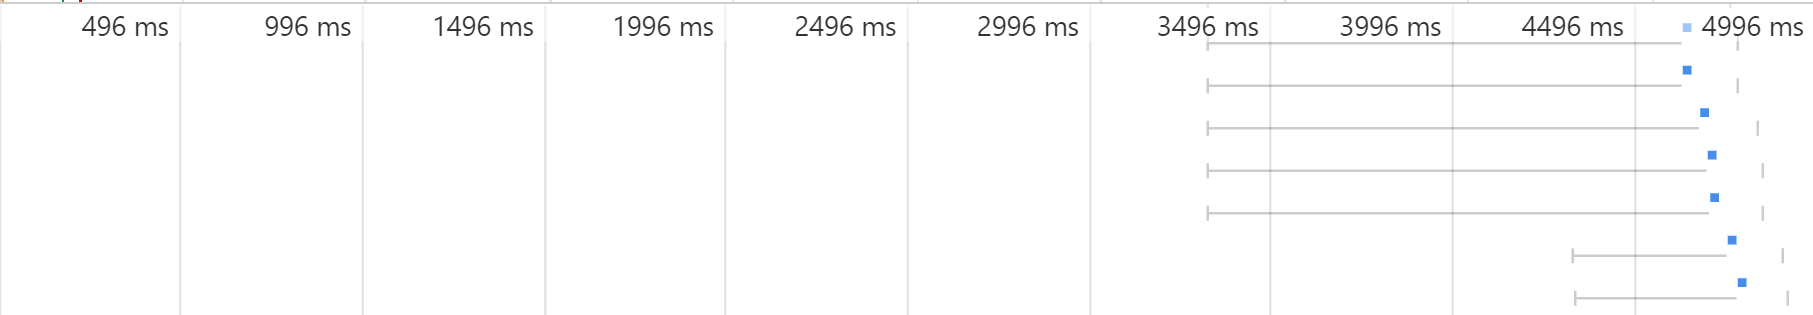
\includegraphics[width=\textwidth]{requestOverlap.png}
  \caption{Überlappen von Ladezyklen}
  \label{requestOverlap}
\end{figure}

Dies ist ein nicht hinnehmbarer Zustand, da ab diesem Zeitpunkt ein kritischer Punkt erreicht ist, ab dem sich alle Requests mit fortlaufender Zeit immer mehr anstauen. Jetzt ist natürlich die Frage, ob diese Limitierung auf Grund der begrenzten Bandbreite und hoher Datenmenge auftritt oder ob der Webserver seine maximale Kapazität erreicht hat. Auf Seiten des Webservers könnte zum einen die Menge an Requests ein limitierender Faktor sein. Zum anderen könnte die Engstelle beim Zugriff auf die Datei mit den Quelldaten liegen, da diese ja für jede Anfrage neu ausgelesen werden muss. Ein Profiling des Server ergab allerdings keine Performanceprobleme. Es standen ungenutzte Threads zur Verfügung und auch die CPU Auslastung war nicht besorgniserregend. Der Durchsatz des Dateisystems lässt sich relativ schwer bestimmen, allerdings wurde es als unwahrscheinlich eingestuft. Klarheit ergab dann der genauere Blick auf einen der am längsten laufende Requests (siehe Abbildung \ref{specificRequest}).

\begin{figure}[H]
  \centering
  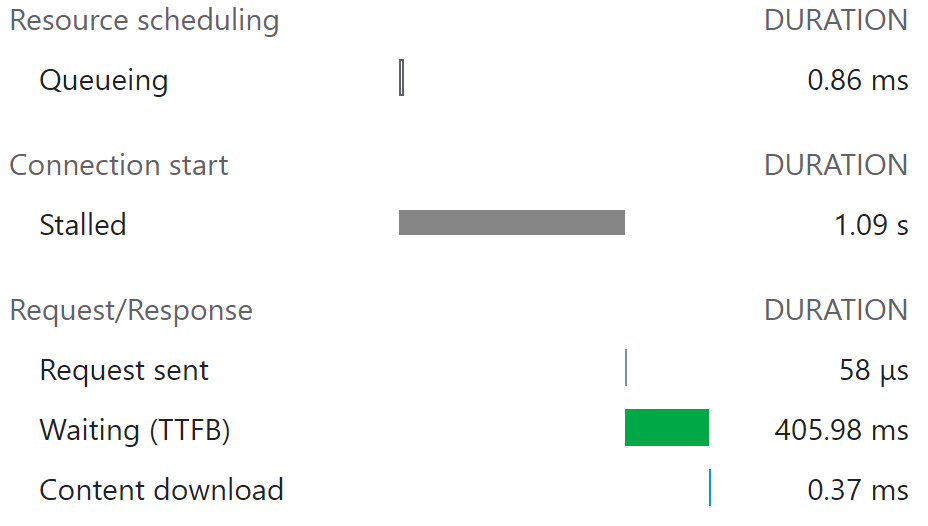
\includegraphics[width=0.7\textwidth]{specificRequest.png}
  \caption{Details des am längsten laufenden Requests}
  \label{specificRequest}
\end{figure}

Dies zeigt, dass der Requests auf Client-Seite sehr lang im Status “Stalled” wartete. Die Zeit, welche mit dem Warten auf die Antwort verbracht wurde, machte dabei nur ein Drittel der Gesamtzeit aus. Eine kurze Recherche zeigte dann, dass die maximale Anzahl an nebenläufigen Requests pro Server im Google Chrome Browser auf sechs limitiert ist. Auch wenn also auf dem Server genügend Ressourcen verfügbar sind, werden diese nicht vollständig ausgeschöpft. Dieses Limit des Browsers lässt sich trotz vielfältiger Feature Requests\footnote{z.B. https://bugs.chromium.org/p/chromium/issues/detail?id=87381} nicht ändern. Als einziger Optimierungspunkt bleibt also die Reduzierung der Laufzeit einzelner Requests auf Serverseite, was nicht trivial umsetzbar ist. Auch könnte man überlegen das HTTP/2 Server Push Feature zu nutzen, mit dem ein Server auf einen Request mit mehr als nur einer Response antworten kann. Somit könnte die Limitierung der Anzahl der Requests umgangen werden. Es ist jedoch unklar, wie aufwändig eine dementsprechende Änderung auf Client- und Serverseite ist.

Auch der Speicherverbrauch im RAM ist deutlich unter den Erwartungen und den Anforderungen (siehe Abbildung \ref{heapSize}). Der Graph zeigt den Speicherplatz im JavaScript Heap über die Zeit an. Die Werte schwanken dabei zwischen 1.1 MB und 9.5 MB.

\begin{figure}[H]
  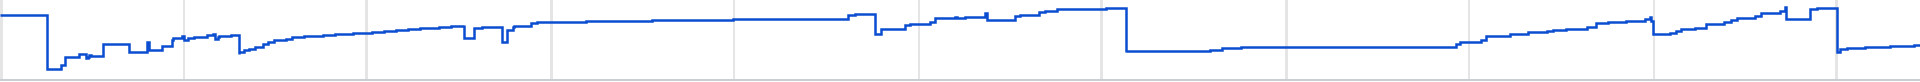
\includegraphics[width=\textwidth]{heapSize.png}
  \caption{Speicherverbrauch im JavaScript Heap über Zeit}
  \label{heapSize}
\end{figure}

Der gesamte RAM und VRAM wurde auch in den Abbildung \ref{memoryAvg} und \ref{memoryMax} mit dem Tool gpu-z ermittelt. Da dies natürlich systemweite Werte darstellt, kann nur mit der Differenz zum Startzeitpunkt gearbeitet werden, um damit einen ungefähren Wert zu erhalten. Dieser Wert ist natürlich auch durch die Benutzung des Browsers an sich verfälscht. Zu Beginn des Tests war der VRAM mit 840 MB und der RAM mit 7740 MB gefüllt. Der Memory Controller Load kann als Indiz genutzt werden, mit welchem Durchsatz Daten auf die GPU geschafft werden können. Seine Auslastung lag zu Anfang bei 2\%. Die GPU Auslastung wurde hier auch nochmal betrachtet, da vorige Tests nur die totale Zeit auf der GPU betrachtet hatten, was nichts darüber aussagt, wie stark sie zu bestimmten Zeiten beansprucht wurde. Da eine GPU eine geteilte Ressource ist, sollte man hierbei auch an andere Anwendungen denken. Sie lag zu Beginn des Tests bei ungefähr 5\%.

\begin{figure}[H]
  \begin{minipage}{0.5\textwidth}
    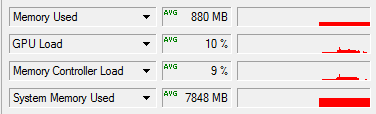
\includegraphics[width=0.95\textwidth]{memoryAvg.png}
    \caption{Durchschnittlicher Speicherverbrauch und Auslastung}
    \label{memoryAvg}
  \end{minipage}
  \begin{minipage}{0.5\textwidth}
    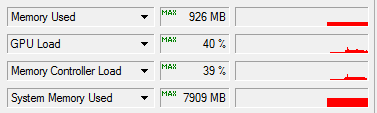
\includegraphics[width=0.95\textwidth]{memoryMax.png}
    \caption{Maximaler Speicherverbrauch und Auslastung}
    \label{memoryMax}
  \end{minipage}
\end{figure}

Auch dieser Test zeigt eine durchschnittliche RAM Nutzung von 108 MB und eine maximale Nutzung von 169 MB, was sich zwar von vorigen Messungen unterschiedet, aber immer noch stark unter den Anforderungen ist. Auch die durchschnittliche VRAM Nutzung von 40 MB und die maximale Nutzung von 86 MB ist nicht zu beanstanden. Interessant ist noch die maximale GPU Auslastung von 40\%, welche deutlich über dem Durchschnitt von 10\% liegt. Dies zeigt aber auch nur, dass selbst zu kritischsten Zeiten die Auslastung völlig vertretbar ist. Und schlussendlich zeigt der maximale Memory Controller Load von 39\%, dass der Datendurchsatz in zukünftigen Projekten mehr als verdoppelt werden könnte.

Als letzten Punkt wurden die Ladezeiten betrachtet, welche auf Grund des asynchronen Natur des Laden schwer zu ermitteln waren. Hier wurde der Ladevorgang um Timing Informationen erweitert um so einen ungefähren Überblick zu erhalten. Nach dem Neuladen der Seite dauerte es dabei 746 ms ab dem onload-Event des Browsers, bis alle Abschnitte in der initialen Ansicht geladen waren. Das onload-Event wird vom Browser gesendet, nachdem alle statischen Ressourcen (HTML, Scripte, Bilder, etc.) geladen wurden. Es trat laut den Entwicklertool nach 112 ms auf, was zu einer gesamten Ladezeit von 858 ms führt. Eine Ladezeit von unter einer Sekunde wurde auf Grund der Datenmenge als vertretbar eingestuft.
\chapter{Fazit}
Mit dieser Arbeit wurde ein

\section{Schlussfolgerungen}

\section{Limitationen}

\section{Ausblick}


\backmatter
\printbibliography
\end{document}